\documentclass[master=cws,masteroption=ci]{kulemt}
\setup{title={Hyperspectrale afbeeldingscompressie via tensordecomposities},
  author={Wouter Baert},
  promotor={Prof.\,dr.\,ir.\ K. Meerbergen \and Dr.\ N. Vannieuwenhoven},
  assessor={Prof. dr. R. Vandebril \and Prof. dr. ir. Ph. Dutr\'e},
  assistant={Dr.\ N. Vannieuwenhoven}}
% De volgende \setup mag verwijderd worden als geen fiche gewenst is.
\setup{filingcard,
  translatedtitle={Hyperspectral image compression via tensor decompositions},
  udc=681.3,
  shortabstract={
Hyperspectrale afbeeldingen zijn afbeeldingen met veel spectrale banden, ten opzichte van de typische drie kleurenbanden in normale afbeeldingen, met toepassingen in bijvoorbeeld voedselverwerking en mijnbouw. Als men alle banden ongecomprimeerd bijhoudt, kan dit voor opslagproblemen zorgen, maar vanwege grote redundantie over de spectrale dimensie kan dit veel effici\"enter. In deze thesis comprimeren we dergelijke afbeeldingen aan de hand van tensordecomposities. Ten eerste is er de Tucker-decompositie, die berekend zal worden met de ST-HOSVD-procedure, versneld door het gebruik van de Gram-matrix. Voor de opslag van de factormatrices gebruiken we een nieuwe techniek, gebaseerd op QR-factorizatie met Householder-reflecties. Hierna volgt de quantisatiefase, waarbij we kiezen voor gelaagde methoden voor zowel de kerntensor als factormatrices, die de inherente structuur van deze objecten benutten. Als laatste stap van de compressie worden de gequantiseerde waarden ge\"encodeerd met een adaptieve strategie, waarbij Gray-codes en Huffman-codes gecombineerd worden. Uiteindelijk worden parameterwaarden voor het volledige algoritme gekozen aan de hand van vaste selectiefuncties, al dan niet gevolgd door een iteratieve verbetering van deze waarden. Ten tweede onderzoeken we ook technieken voor het comprimeren van hyperspectrale afbeeldingen als hervormde 5D-tensoren. De \textit{tensor-train}-decompositie blijkt beter te werken dan de Tucker-decompositie voor het comprimeren van dergelijke hoog-dimensionale tensoren. Daarom ontwikkelen we hiervoor een eigen compressie-algoritme, analoog aan Tucker-gebaseerde compressie. Op het einde vergelijken we de resultaten van onze twee compressie-algoritmen met elkaar, enkele algemene \textit{lossy} compressiemethoden en een algoritme uit de literatuur. Onze resultaten zien er beloftevol uit: zo kan men met onze tensor-train-gebaseerde compressie op typische datasets compressiefactoren van ordegrootte 100 tot 1000 halen bij fouten die insignificant zijn voor visualisatie-toepassingen.
}}
% Verwijder de "%" op de volgende lijn als je de kaft wil afdrukken
%\setup{coverpageonly}
% Verwijder de "%" op de volgende lijn als je enkel de eerste pagina's wil
% afdrukken en de rest bv. via Word aanmaken.
%\setup{frontpagesonly}

% Kies de fonts voor de gewone tekst, bv. Latin Modern
\setup{font=lm}

% Hier kun je dan nog andere pakketten laden of eigen definities voorzien

% Tenslotte wordt hyperref gebruikt voor pdf bestanden.
% Dit mag verwijderd worden voor de af te drukken versie.
%\usepackage[pdfusetitle,colorlinks,plainpages=false]{hyperref}
\usepackage[pdfusetitle,plainpages=false,hidelinks]{hyperref}

% Eigen toevegingen
%\setup{coverpageonly}
\maxsecnumdepth{subsubsection}
\usepackage{float}
\usepackage{amsmath}
\usepackage{amsfonts}
\usepackage{verbatim}
\usepackage[]{algorithm2e}
\usepackage{hhline}
\usepackage{subcaption}
\usepackage{multirow}
\usepackage{xcolor}
\usepackage[mathscr]{euscript}
\setcounter{MaxMatrixCols}{20}

% Listings stuff
\usepackage{listings}
\lstset{
	basicstyle=\tiny,
	keywordstyle=\color{blue},
	stringstyle=\color{orange},
	commentstyle=\color{red},
	showstringspaces=false,
	numbers=left,
	stepnumber=2,
	numbersep=5pt,
	frame=single,
	breaklines=true,
	tabsize=2,
	breakatwhitespace=true,
	morecomment=[l]{//}
}
\lstdefinestyle{Python}{language=Python}
\lstdefinestyle{C}{language=C}

%%%%%%%
% Om wat tekst te genereren wordt hier het lipsum pakket gebruikt.
% Bij een echte masterproef heb je dit natuurlijk nooit nodig!
\IfFileExists{lipsum.sty}%
 {\usepackage{lipsum}\setlipsumdefault{11-13}}%
 {\newcommand{\lipsum}[1][11-13]{\par Hier komt wat tekst: lipsum ##1.\par}}
%%%%%%%

%\includeonly{hfdst-n}
\begin{document}

\begin{preface}
In de eerste plaats wil ik mijn copromotor en begeleider, dr. Nick Vannieuwenhoven bedanken. Doorheen onze vele vergaderingen gaf hij een goede richting aan mijn onderzoek en verleende hij talrijke nuttige tips voor mijn werk. Ook bij het schrijven van deze tekst ontving ik regelmatig uitgebreide en snelle feedback. Zonder zijn begeleiding was deze thesis niet tot stand gekomen, dus hiervoor mijn oprechte dank.\\

Daarnaast bedank ik ook mijn promotor, prof. dr. ir. Karl Meerbergen, voor zijn bijdrage aan de initi\"ele ori\"entering van deze thesis, feedback bij de tussentijdse presentatie en andere hulp. Verder gaat mijn dank eveneens uit naar alle leden van de jury voor het lezen van deze tekst, die uiteindelijk eerder lang geworden is, en het beoordelen van deze thesis.\\

Ten slotte wil ik ook even een aantal medestudenten bedanken, met name Kristof Achten, Michiel Bollen, Sven Cuyt en Arno Coomans. Hun solidariteit en gezelschap in het Departement Computerwetenschappen gedurende de afgelopen weken, waarin er voltijds aan deze thesis werd geschreven, heb ik erg geapprecieerd.
\end{preface}

\tableofcontents*

\begin{abstract}
Hyperspectrale afbeeldingen zijn afbeeldingen met veel spectrale banden, ten opzichte van de typische drie kleurenbanden in normale afbeeldingen. Dergelijke fijne metingen hebben toepassingen in bijvoorbeeld voedselverwerking en mijnbouw. Als men echter alle banden ongecomprimeerd probeert bij te houden, kan dit voor geheugenproblemen zorgen, maar vanwege grote redundantie over de spectrale dimensie kan men deze data veel effici\"enter opslaan.\\

In deze thesis comprimeren we dergelijke hyperspectrale afbeeldingen aan de hand van tensordecomposities. Ten eerste leggen we onze focus op de Tucker-decompositie, die berekend zal worden met de ST-HOSVD-procedure. We onderzoeken enkele optimisaties hiervoor, maar alleen de Gram-matrix-methode blijkt effectief. Voor de opslag van de factormatrices gebruiken we een nieuwe techniek, gebaseerd op het QR-factorizatie-algoritme met Householder-reflecties. Hierna volgt de quantisatiefase, waarbij we kiezen voor gelaagde methoden voor zowel de kerntensor als factormatrices, die de inherente structuur van deze objecten benutten. Als laatste stap van de compressie worden de gequantiseerde waarden ge\"encodeerd en \textit{lossless} gecomprimeerd aan de hand van het Deflate-algoritme. We gebruiken hiervoor adaptieve encodering, waarbij zowel Gray-codes als Huffman-codes gecombineerd worden om de totale opslag te verminderen. Ten slotte worden parameterwaarden voor het volledige algoritme gekozen aan de hand van vaste selectiefuncties, al dan niet gevolgd door een iteratieve verbetering van deze waarden.\\

Ten tweede onderzoeken we ook technieken voor het comprimeren van hyperspectrale afbeeldingen als hervormde 5D-tensoren. De Tucker-decompositie blijkt slechter te werken na hervorming, maar een andere decompositie, de \textit{tensor train}, is beter in het comprimeren van dergelijke hoog-dimensionale tensoren. Daarom ontwikkelen we voor tensor trains een eigen compressie-algoritme, analoog aan Tucker-gebaseerde compressie met kleine aanpassingen.\\

Op het einde van deze tekst vergelijken we de resultaten van onze twee compressie-algoritmen met elkaar, enkele algemene \textit{lossy} compressiemethoden en een algoritme uit de literatuur, zowel op vlak van compressiefactor, -fout, -tijd en decompressietijd. Onze resultaten zien er beloftevol uit: zo kan men met onze tensor-train-gebaseerde compressie op typische datasets compressiefactoren van ordegrootte 100 tot 1000 halen bij fouten die insignificant zijn voor visualisatie-toepassingen.
\end{abstract}

% Een lijst van figuren en tabellen is optioneel
%\listoffigures
%\listoftables
% Bij een beperkt aantal figuren en tabellen gebruik je liever het volgende:
%\listoffiguresandtables
% De lijst van symbolen is eveneens optioneel.
% Deze lijst moet wel manueel aangemaakt worden, bv. als volgt:]
%\chapter{Lijst van afkortingen en symbolen}
%\section*{Afkortingen}
%\begin{flushleft}
%  \renewcommand{\arraystretch}{1.1}
%  \begin{tabularx}{\textwidth}{@{}p{12mm}X@{}}
%    LoG   & Laplacian-of-Gaussian \\
%    MSE   & Mean Square error \\
%    PSNR  & Peak Signal-to-Noise ratio \\
%  \end{tabularx}
%\end{flushleft}
%\section*{Symbolen}
%\begin{flushleft}
%  \renewcommand{\arraystretch}{1.1}
%  \begin{tabularx}{\textwidth}{@{}p{12mm}X@{}}
%    42    & ``The Answer to the Ultimate Question of Life, the Universe,
%            and Everything'' volgens de \cite{h2g2} \\
%    $c$   & Lichtsnelheid \\
%    $E$   & Energie \\
%    $m$   & Massa \\
%    $\pi$ & Het getal pi \\
%  \end{tabularx}
%\end{flushleft}

% Nu begint de eigenlijke tekst
\mainmatter

\chapter{Inleiding}
\label{hoofdstuk:inleiding}

We zijn allemaal vertrouwd met afbeeldingen. Deze bestaan uit een 2D-rooster van pixels, waarbij elke pixel typisch bestaat uit drie kleurenwaarden die de intensiteit van rood, groen en blauw licht in de pixel beschrijven. Om deze reden zeggen we ook dat een normale afbeelding drie \textit{spectrale banden} bevat. Hiermee kan men het spectrum van zichtbaar licht goed benaderen op een manier die door het menselijk zicht waargenomen wordt op quasi identieke wijze als het originele beeld.\\

Voor sommige toepassingen is het echter ook nuttig om het gemeten lichtspectrum onder te verdelen in meer dan drie banden. In dit geval spreken we van \textit{hyperspectrale} afbeeldingen. Zo voert de AVIRIS-sensor (\textit{Airborne Visible/InfraRed Imaging Spectrometer}) van NASA \cite{ref:aviris_website} metingen uit in 224 banden over het zichtbare spectrum en een deel van het infrarood-spectrum. Toepassingen hiervan bestaan onder meer uit het opvolgen van de staat van landbouwgewassen \cite{ref:tilling}, het detecteren van afwijkingen in voedsel \cite{ref:higgins} en het in kaart brengen van mineralen op basis van luchtfoto's \cite{ref:resmini}.\\

Wanneer men hyperspectrale afbeeldingen wil opslaan, stoot men echter tegen een probleem. Een typische AVIRIS-dataset bevat miljoenen pixels en kan in een ongecomprimeerd formaat tientallen gigabytes groot zijn. Het is dus erg nuttig om compressietechnieken hiervoor te ontwikkelen.\\

In figuur \ref{fig:cuprite-bands} tonen we verschillende reeksen spectrale banden van een hyperspectrale luchtfoto van Cuprite (Nevada) in de Verenigde Staten. Er zijn significante verschillen zichtbaar tussen de banden, maar de structuur blijft duidelijk hetzelfde. Op spectraal niveau is er dus erg veel redundantie en dit kunnen we benutten om dezelfde data met minder geheugen voor te stellen.

\newpage
\begin{figure}[H]
\centering
\begin{subfigure}{0.48\textwidth}
  \centering
  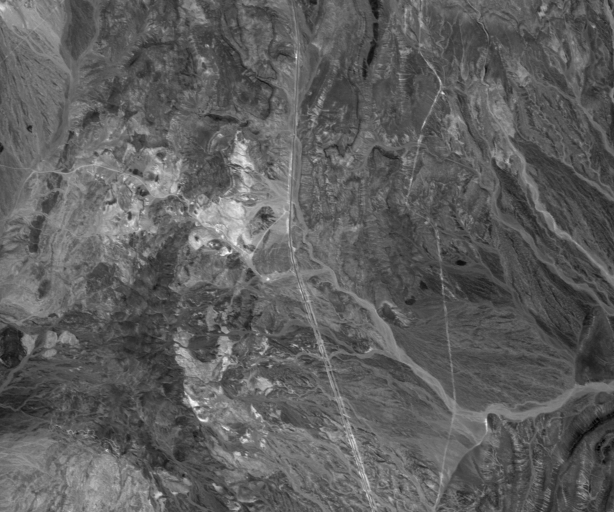
\includegraphics[width=0.95\linewidth]{images/cuprite_bands_0-32.png}
  \caption{Banden 0-31}
\end{subfigure}
\begin{subfigure}{0.48\textwidth}
  \centering
  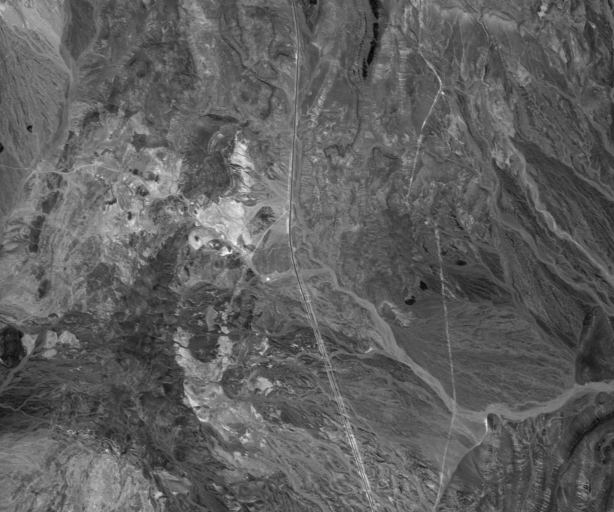
\includegraphics[width=0.95\linewidth]{images/cuprite_bands_32-63.png}
  \caption{Banden 32-62}
\end{subfigure}
\\
\begin{subfigure}{0.48\textwidth}
  \centering
  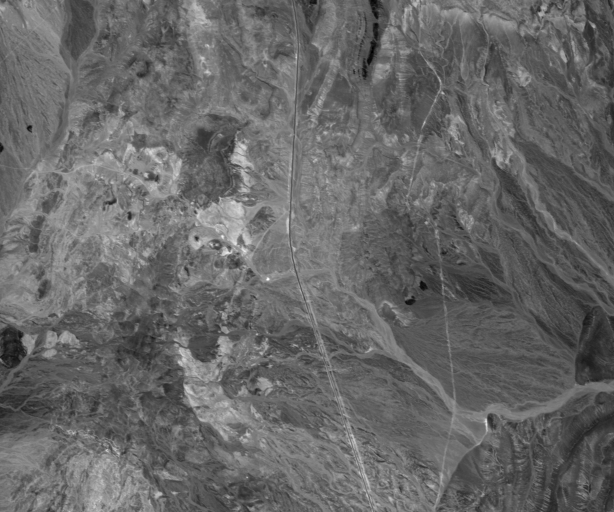
\includegraphics[width=0.95\linewidth]{images/cuprite_bands_63-95.png}
  \caption{Banden 63-94}
\end{subfigure}
\begin{subfigure}{0.48\textwidth}
  \centering
  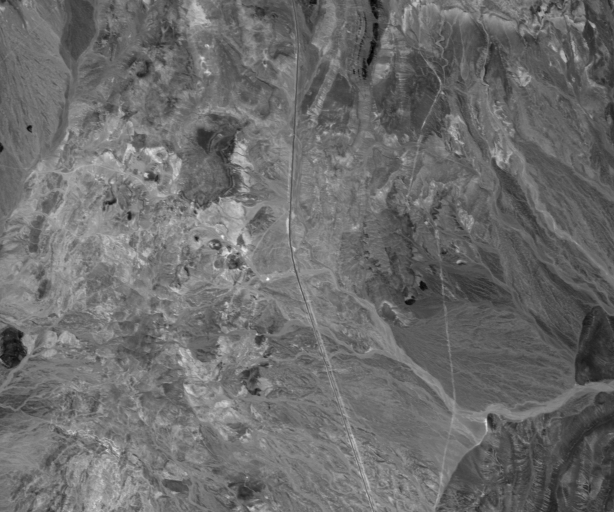
\includegraphics[width=0.95\linewidth]{images/cuprite_bands_95-127.png}
  \caption{Banden 95-126}
\end{subfigure}
\\
\begin{subfigure}{0.48\textwidth}
  \centering
  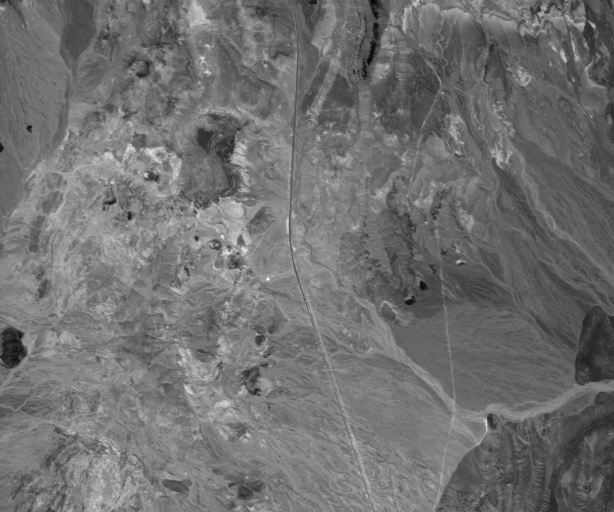
\includegraphics[width=0.95\linewidth]{images/cuprite_bands_127-158.png}
  \caption{Banden 127-157}
\end{subfigure}
\begin{subfigure}{0.48\textwidth}
  \centering
  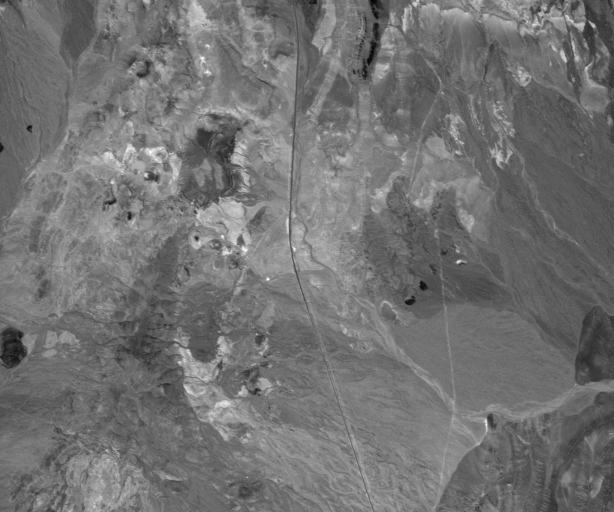
\includegraphics[width=0.95\linewidth]{images/cuprite_bands_158-190.png}
  \caption{Banden 158-189}
\end{subfigure}
\caption{Verschillende delen van een hyperspectrale afbeelding van Cuprite (VS) \cite{ref:ehu_aviris_cuprite}. We tonen hier slechts de 190 banden die overblijven na de voorverwerking die besproken zal worden in hoofdstuk \ref{hoofdstuk:methodologie}.}
\label{fig:cuprite-bands}
\end{figure}
\newpage

Wiskundig gezien kan men de 3D data van een hyperspectrale afbeelding beschouwen als een \textit{tensor}. Daarnaast kennen we vanuit de lineaire algebra de afgeknotte singulierewaardenontbinding, waarmee men met een beperkte fout matrices in een verkleind formaat kan opslaan. Aangezien men met deze decompositie effici\"ent de belangrijkste spectrale signaturen in een hyperspectrale afbeelding kan opsporen, zullen we in deze thesis compressie onderzoeken via tensordecomposities die hierop gebaseerd zijn.\\

Eerst zullen we in hoofdstuk \ref{hoofdstuk:achtergrond} enkele zaken herhalen en nieuwe concepten aanhalen zodat alle vereiste voorkennis besproken is. Het gaat hier onder andere over het verschil tussen \textit{lossless} en \textit{lossy} compressie, tensoren en hun operaties, de singulierewaardenontbinding en de Tucker-decompositie. Aan het einde van dit hoofdstuk volgt ook nog een korte literatuurstudie over hyperspectrale afbeeldingscompressie.\\

In hoofdstuk \ref{hoofdstuk:methodologie} bespreken we de methodologie achter de experimenten die we zullen uitvoeren in de volgende hoofdstukken. Daarna volgt hoofdstuk \ref{hoofdstuk:tucker} over compressie gebaseerd op de Tucker-decompositie, waarin het grootste deel van ons eigen onderzoek behandeld wordt. Hierin zullen we onderzoeken hoe we de singulierewaardenontbinding in bepaalde omstandigheden sneller kunnen berekenen, gevolgd door een analyse van de volgende stappen van de compressie: orthogonaliteitscompressie, quantisatie en encodering. Op deze manier bekomen we uiteindelijk een volledig Tucker-gebaseerd compressie-algoritme. Ten slotte bespreken we ook nog technieken om goede parameters te selecteren voor dit algoritme.\\

Hierna komt hoofdstuk \ref{hoofdstuk:hervorming}, waarin we de hyperspectrale afbeeldingen hervormen naar vijf dimensies en onderzoeken of er hiervoor betere compressiemethoden bestaan. We analyseren zowel het effect van Tucker-gebaseerde compressie als compressie gebaseerd op een nieuwe decompositie: \textit{tensor trains}.\\

In hoofdstuk \ref{hoofdstuk:resultaten} zullen we de uiteindelijke resultaten van onze compressiemethoden bespreken. Hierbij vergelijken we deze methoden zowel onderling als met enkele algemene compressie-algoritmen en een algoritme uit de literatuur, waarna we het hoofdstuk afsluiten met een aantal voorbeelden van gecomprimeerde hyperspectrale afbeeldingen.\\

Ten slotte eindigen we deze thesis met hoofdstuk \ref{hoofdstuk:besluit}, waarin we de conclusies van ons werk samenvatten. Hiernaast wordt er ook aandacht besteed aan mogelijke pistes voor verder onderzoek om onze compressie-algoritmen te verbeteren.

\chapter{Achtergrondinformatie}
\label{hoofdstuk:achtergrond}

\begin{itemize}
\item Hyperspectrale afbeeldingen
\item compressie: lossless en lossy (JPEG)
\item tensoren, n-mode product
\item Tucker, T-HOSVD
\item ST-HOSVD: algemeen, modevolgorde
\item Deflate
\item JPEG
\end{itemize}

\chapter{Methodologie}
\label{hoofdstuk:methodologie}

We zullen zowel bij het vergelijken van de uiteindelijke algoritmes in hoofdstuk \ref{hoofdstuk:resultaten} als bij het vergelijken van verschillende technieken en parameterwaarden in hoofdstuk \ref{hoofdstuk:tucker} en hoofdstuk \ref{hoofdstuk:hervorming} experimenten uitvoeren om onze conclusies te staven. Om deze reden zullen we eerst alle nodige context voor deze experimenten beschrijven in dit hoofdstuk.

\section{Algemeen}
Om rekening te houden met variantie, zullen tijdsmetingen in deze tekst uitgemiddeld worden over 10 experimenten, tenzij anders vermeld. Technisch gezien zijn de resultaten van stochastische algoritmen ook niet compleet deterministisch, maar aangezien de variantie hierop vaak minimaal is zal de nood aan een grotere steekproef geval per geval behandeld worden. Daarnaast zullen tijdsmetingen ook uitgedrukt worden in CPU-tijd.

\section{Hardware}
Tenzij anders vermeld werden de tijdsmetingen in deze tekst uitgevoerd op \'e\'en core van een Intel(R) Core(TM) i7-4700HQ CPU @ 2.40GHz processor met 6GB RAM.

\section{Compressiefactor}

De compressiefactor is een belangrijke variabele die we zullen gebruiken in deze thesis. Hiermee hebben we het over de verhouding tussen de grootte van de originele, ongecomprimeerde 3D-tensor (dus bijvoorbeeld voor een $100 \times 100 \times 10$ tensor bestaande uit 16-bit integers is dit 200000 bytes) en de grootte van de gecomprimeerde versie (met als datatype voor niet-gehele getallen 32-bit floats, tenzij anders vermeld). Dit is echter een erg simpel formaat en niet altijd de beste manier om deze data op te slaan. Men moet er dus rekening mee houden dat men alleen al door de rauwe data op te slaan in een Zip-archief een compressiefactor van bijvoorbeeld 1.35 kan bekomen. Bijgevolg dient deze factor vooral relatief bekeken te worden, om verschillende compressietechnieken met elkaar te kunnen vergelijken.\\

Verder zal het geheugengebruik van metadata (onder meer afmetingen van tensoren, compressieparameters en modevolgorde) verwaarloosd worden, aangezien dit veel kleiner is dan de benodigde opslagruimte voor tensoren en matrices. Concreet betekent dit dat we alleen geheugenruimte zullen meetellen van objecten die in een zekere zin groeien met de grootte van de invoer, behalve als deze groeien met het aantal dimensies van de tensoren waarmee we werken (aangezien dit in de praktijk toch heel beperkt is).

\section{Compressiefout}

Idealiter meet men de fout ge\"introduceerd door compressie in functie van de beoogde toepassing van de gedecomprimeerde data. Zo heeft men bij het ontwerp van belangrijke compressiemethoden als JPEG \cite{ref:jpeg} (normale afbeeldingen) en x264 \cite{ref:x264} (video's) rekening gehouden met de eigenschappen van de menselijke waarneming. Om praktische redenen zullen we echter werken met de relatieve fout, simpelweg gedefinieerd als:
\[
\text{relatieve fout} = \frac{||\text{gereconstrueerde tensor} - \text{originele tensor}||_F}{||\text{originele tensor}||_F}
\]

\section{Implementatie}

De implementatie van de besproken algoritmen gebeurde in Python, waarbij het zware rekenwerk werd uitgevoerd via library calls, voornamelijk aan de hand van NumPy, SciPy en zlib. Hierbij zijn ook alternatieve strategie\"en getest (zoals het al dan niet minimaliseren van transposities, het gebruik van \texttt{numpy.einsum}, ...), waarbij telkens de meest performante werd gekozen. Deze keuzes zullen weinig behandeld worden in deze tekst vanwege de sterke afhankelijkheid van de gekozen programmeertaal. Desalniettemin kan het dat er nog steeds merkbare ineffici\"enties in de implementatie zijn.\\

Om enkele verschillende encoderingen effici\"ent te kunnen uitvoeren, hebben we niet alleen de Python-module \texttt{bitarray} \cite{ref:bitarray} gebruikt, maar deze ook uitgebreid met enkele methodes (zie sectie \ref{sec:encodering} voor meer informatie). Deze code werd, zoals de rest van de module, in C geschreven voor performantie.\\

Zoals eerder vermeld, zullen de belangrijkste stukken broncode toegevoegd worden als bijlage. Om de lengte van deze tekst te beperken, zal niet de volledige code aanwezig zijn in deze bijlagen, maar deze is beschikbaar via de \textit{repository}: \url{https://github.com/Wout12345/hyperspectral-image-compression-co}

\section{Datasets}

Om een idee te krijgen van de effici\"entie van de verschillende compressietechnieken, moet men gebruik maken van echte hyperspectrale afbeeldingen. Hieronder volgen enkele voorbeelden met hun bijbehorende eigenschappen. De afbeeldingen zijn slechts een 2D-voorstelling van de hyperspectrale data, verkregen door alle frequentiekanalen bij elkaar op te tellen en deze sommen voor te stellen met grijswaarden. Dit zijn ook telkens voorstellingen van de finale datasets waarmee we werken, zonder eventuele verwijderde spatiale en spectrale banden.\\

Bij de voorverwerking zullen we vaak bepaalde spectrale banden weglaten indien blijkt dat deze artefacten bevatten (onder meer banden met waarde 0, banden met veel te hoge, willekeurig verdeelde intensiteiten en naburige banden). Op spatiaal vlak zullen we soms de afmetingen naar beneden afronden tot het dichtsbijzijnde kwadraat; hierdoor kan men deze assen eventueel later nog makkelijk reshapen. Verder is het ook in sommige gevallen nodig om een geroteerde in plaats van as-gealigneerde rechthoek te selecteren. Hierbij vallen de roosterpunten in het nieuwe assenstelsel niet exact op oude roosterpunten en zal de nieuwe dataset gereconstrueerd worden door bilineair te interpoleren \cite{ref:bilinear_interpolation} over de twee spatiale assen.\\

Omdat de geproduceerde bestanden te groot zijn om in bijlage toe te voegen en deze voorverwerking niet triviaal is om formeel te beschrijven, hebben we de code van de voorverwerker toegevoegd in bijlage \ref{app:voorverwerker}. Men kan deze combineren met de originele data van de corresponderende bronnen om dezelfde datasets te reproduceren.

\subsection{Indian Pines}

\begin{figure}[H]
  \centering
  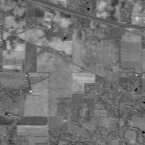
\includegraphics[scale=1]{images/indian_pines_sum.png}
  \caption{Indian Pines, VS. Bron: AVIRIS \cite{ref:ehu_aviris_indian_pines}}
  \label{fig:indian_pines_sum}
\end{figure}

\textbf{Spatiale dimensies:} $145 \times 145$\\
\textbf{Spectrale dimensie:} 220\\
\textbf{Voorverwerking:} Geen.

\newpage
\subsection{Cuprite}

\begin{figure}[H]
  \centering
  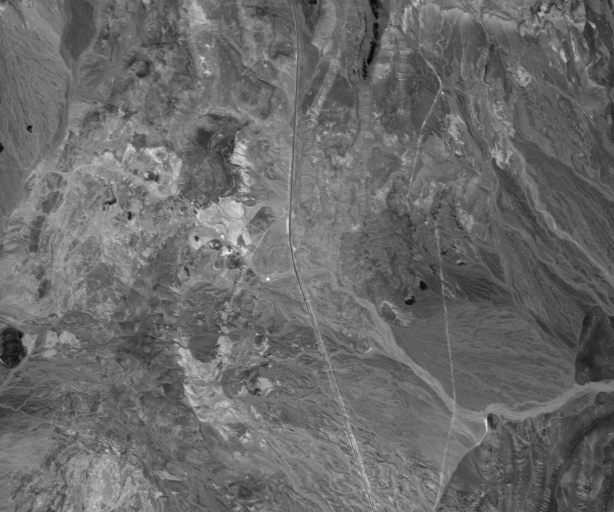
\includegraphics[scale=0.5]{images/cuprite_sum.png}
  \caption{Cuprite, VS. Bron: AVIRIS \cite{ref:ehu_aviris_cuprite}}
  \label{fig:cuprite_sum}
\end{figure}

\textbf{Spatiale dimensies:} $512 \times 614$\\
\textbf{Spectrale dimensie:} 190\\
\textbf{Voorverwerking:} De originele spectrale dimensie was 224, maar banden 0-3, 106-113, 152-168 en 219-223 werden verwijderd.

\newpage
\subsection{Pavia Centre}

\begin{figure}[H]
  \centering
  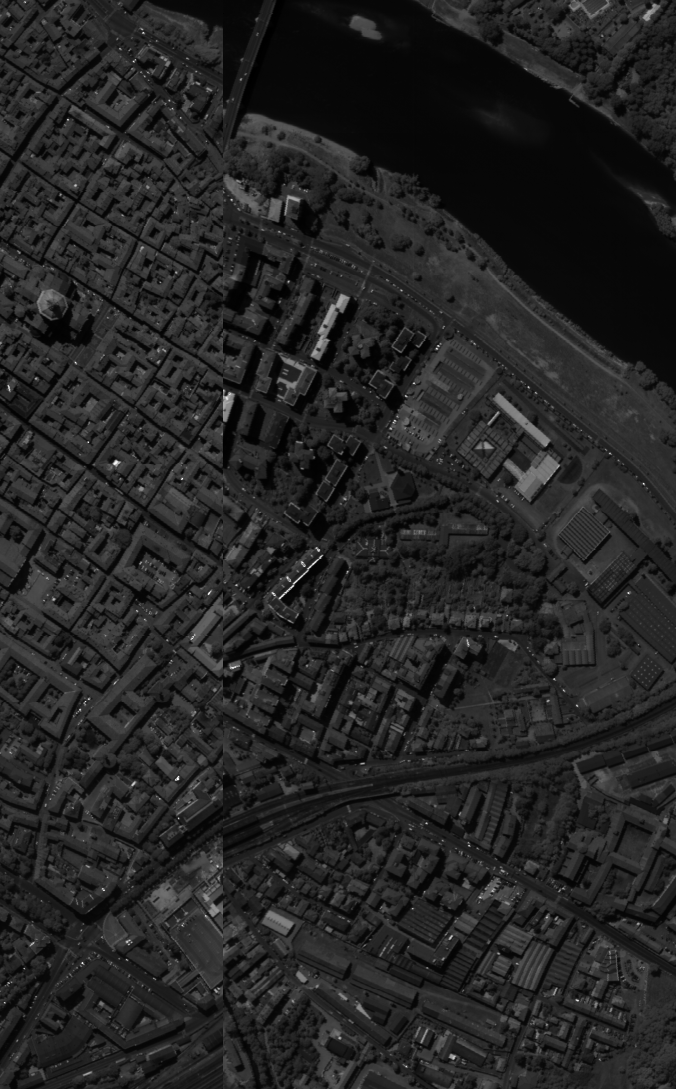
\includegraphics[scale=0.4]{images/pavia_sum.png}
  \caption{Pavia Centre, Itali\"e. Bron: ROSIS \cite{ref:ehu_rosis}}
  \label{fig:pavia_sum}
\end{figure}

\textbf{Spatiale dimensies:} $1089 \times 676$\\
\textbf{Spectrale dimensie:} 102\\
\textbf{Voorverwerking:} De download van de EHU \cite{ref:ehu_rosis} heeft al een reeks spatiale banden zonder informatie weggelaten en heeft spatiale dimensies $1096 \times 715$. Hiervan selecteerden we de pixels met de laagste indices. De weggelaten rijen en kolommen zouden zich dus onder en rechts van de afbeelding hierboven bevinden.

\newpage
\subsection{Mauna Kea}

\begin{figure}[H]
\centering
\begin{subfigure}{.5\textwidth}
  \centering
  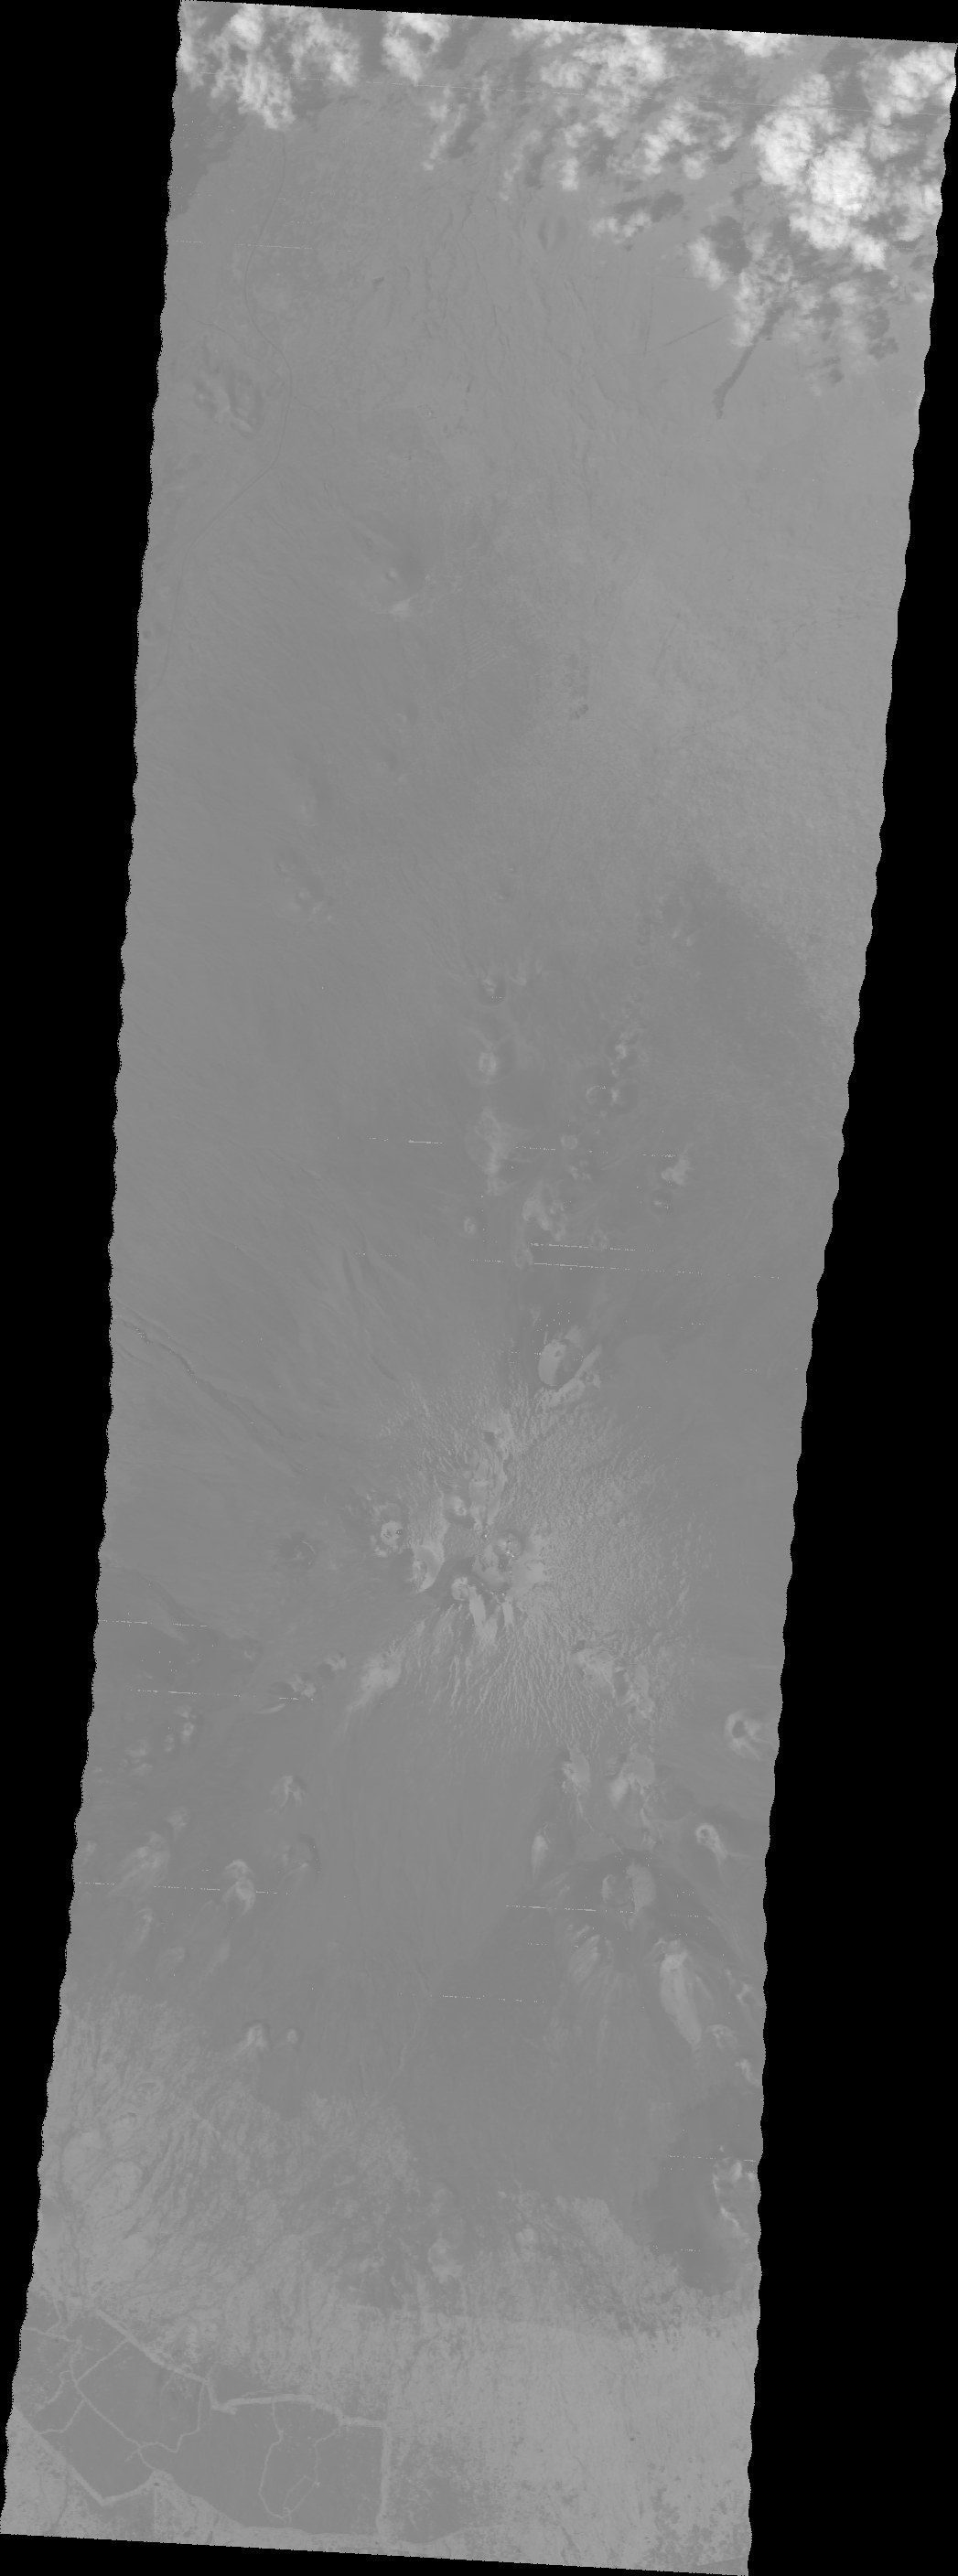
\includegraphics[scale=0.14]{images/mauna_kea_raw_sum.png}
  \caption{Origineel}
\end{subfigure}%
\begin{subfigure}{.5\textwidth}
  \centering
  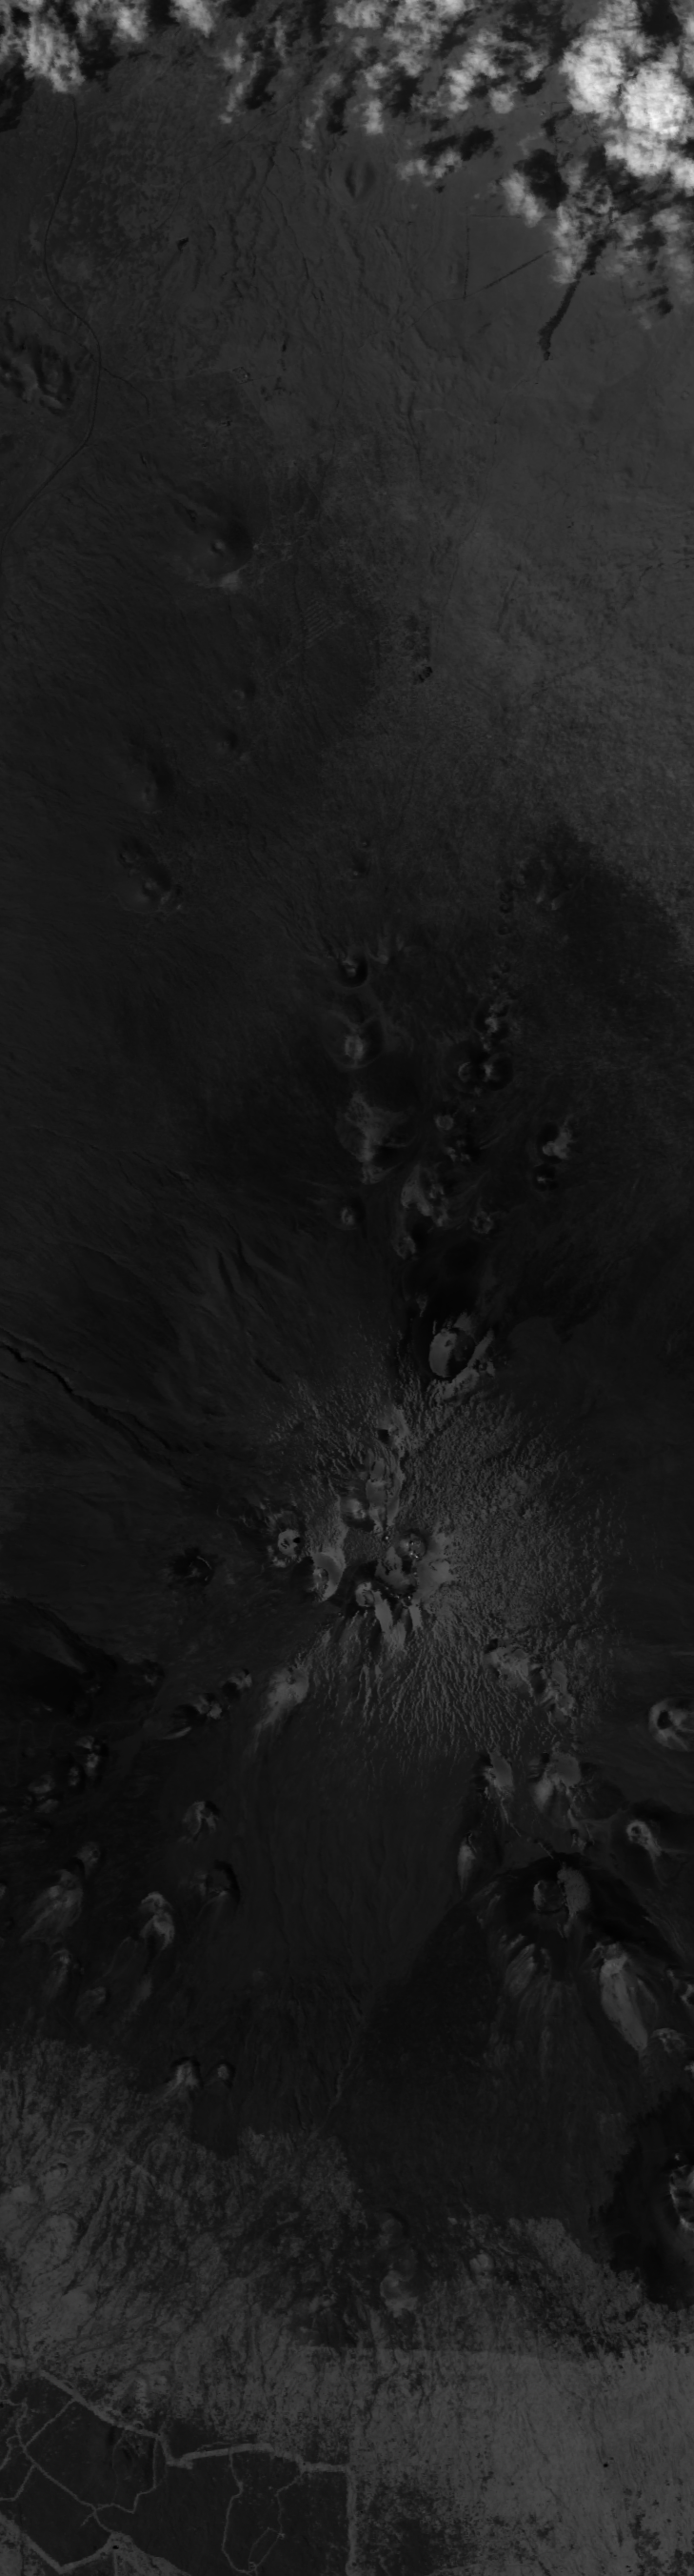
\includegraphics[scale=0.14]{images/mauna_kea_sum.png}
  \caption{Na voorverwerking}
\end{subfigure}
\caption{Mauna Kea, VS. Bron: AVIRIS \cite{ref:aviris}}
\label{fig:mauna_kea}
\end{figure}

\textbf{Spatiale dimensies:} $2704 \times 729$\\
\textbf{Spectrale dimensie:} 199\\
\textbf{Voorverwerking:} Op spatiaal vlak werd een rechthoek geselecteerd, beginnend in (40, 240) en 4.07 graden wijzerzin gedraaid ten opzichte van het originele assenstelsel. Op spectraal vlak werden van de 224 originele banden de banden 0-1, 103, 107-113 en 153-167 verwijderd. Hierna werden alle waarden verschoven en geschaald zodat het bereik ervan exact overeenkomt met dat van unsigned 16-bit integers, het data type dat ook voor de andere datasets gebruikt werd.
\chapter{De Tuckerdecompositie}
\label{hoofdstuk:tucker}

In dit hoofdstuk zullen we verder bouwen op het standaard ST-HOSVD-algoritme om tot een volledig Tucker-gebaseerd compressie-algoritme te komen. Hierbij zullen we de ST-HOSVD versnellen zonder dat de compressie hieronder lijdt, methoden bekijken om orthogonale matrices verder te comprimeren, technieken vergelijken voor het quantizeren van de kerntensor en factormatrices en ten slotte alles lossless comprimeren met Deflate.

\section{Versnellen van de ST-HOSVD}

Hoewel de focus van deze tekst ligt op de afweging tussen de compressiefactor en compressiefout, is het ook nuttig om te kijken naar de compressietijd. In deze sectie zullen enkele technieken besproken worden om de ST-HOSVD te versnellen zonder de fout merkbaar te verhogen.

\subsection{Modevolgorde}

Zoals eerder besproken is het bij de ST-HOSVD van groot belang voor de performantie om de verschillende modes in de juiste volgorde te verwerken. Aangezien we werken met hyperspectrale afbeeldingen, zal de spectrale mode typisch veel beter comprimeren dan de spatiale modes. Ter illustratie: bij het uitvoeren van het standaard ST-HOSVD-algoritme met relatieve doelfout 0.025, comprimeert Cuprite van rang $512 \times 614 \times 190$ naar de volgende rang:
\begin{table}[H]
\centering
\begin{tabular}{|l|l|}
\hline
Modevolgorde & Compressierang \\ \hline
\input{data/modevolgorde.tex}
\end{tabular}
\end{table}
De spectrale dimensie is dus zeker de best comprimeerbare en zal bijgevolg vanaf nu eerst verwerkt worden, gevolgd door de spatiale dimensies (gerangschikt van groot naar klein).

\subsection{Versnellen van de SVD}

\subsubsection{Gram-matrix}

Een belangrijke eigenschap van de SVD is diens verband met de eigenwaardenontbinding. Wanneer $A = U \Sigma V^T$, dan vormen $U$ en $\Sigma^2$ namelijk respectievelijk de eigenvectoren en eigenwaarden van $A A^T$, ook wel bekend als de Gram-matrix van de rijen van $A$ \cite{ref:svd}. Als $A \in \mathbb{R}^{m \times n}$ met $m \ll n$, dan is $A A^T \in \mathbb{R}^{m \times m}$, wat leidt tot een veel snellere eigenwaardenontbinding dan wanneer men de SVD toepast op de volledige matrix. Bij deze methode moet men wel eerst een matrixvermenigvuldiging uitvoeren met complexiteit $O(m^2 n)$, wat van dezelfde orde is als het normaal berekenen van de SVD \cite{ref:svd}, maar dit kan in de praktijk nog steeds erg nuttig zijn aangezien de matrixvermenigvuldiging een relatief eenvoudige operatie is die al sterk geoptimaliseerd is in libraries als LAPACK \cite{ref:lapack}. Verder kan deze aanpak numerieke problemen opleveren omdat we eerst de invoerdata met zichzelf vermenigvuldigen en op het einde de vierkantswortels trekken van de eigenwaarden, wat de precisie verlaagt, maar in deze toepassing hoeft dit geen probleem te zijn aangezien we de SVD sterk afknotten en dit de grootste fout zal veroorzaken. Voor ons zijn fouten van deze grootte dus irrelevant.\\

Een klein nadeel van deze techniek is dat we de matrix $V$ niet meteen hebben zoals bij het berekenen van een SVD. De matricizatie van de gecomprimeerde data $X_k$ (met compressierang $k$) moet nu dus bepaald worden als $X_k := U_k^T X$ (complexiteit $O(kmn)$) in plaats van $X_k := \Sigma_k V_k$ (complexiteit $O(kn)$), wat een hogere complexiteit heeft, maar dit is slechts een matrixvermenigvuldiging dus dit kost niet zo veel tijd meer.\\

\begin{table}[H]
\centering
\begin{tabular}{|l|l|l|}
\hline
Methode & Relatieve fout & Compressietijd (s)\\ \hline
\input{data/gram-matrix.tex}
\end{tabular}
\caption{Vergelijking tussen de standaard ST-HOSVD en de methode met de Gram-matrix voor Cuprite met relatieve doelfout 0.025 (uitgemiddeld over 10 experimenten).}
\end{table}
Dit voorbeeld bevestigt dus dat deze methode een grote versnelling kan opleveren zonder enige significante fout te introduceren.

\subsubsection{Gram-matrix met QR-decompositie}

Om de eventuele fout die veroorzaakt wordt door te werken met de Gram-matrix te verkleinen, is het een gekende techniek om eerst een QR-decompositie van $A^T$ berekenen. Hoewel we eerder bespraken dat deze fout voor onze toepassing minimaal is, is deze techniek in het algemeen interessant om naar te kijken indien het niet veel extra rekentijd kost. In dit geval berekent men eerst $A^T = QR$ en gebruikt men dan de matrix $A A^T = R^T Q^T Q R = R^T R$ in plaats van $A A^T$ als invoer voor de eigenwaardenontbinding.\\

\begin{table}[H]
\centering
\begin{tabular}{|l|l|l|}
\hline
Methode & Relatieve fout & Compressietijd (s)\\ \hline
\input{data/gram-matrix-qr.tex}
\end{tabular}
\caption{Vergelijking tussen de methode met de Gram-matrix met en zonder QR-decompositie voor Cuprite met relatieve doelfout 0.025 (uitgemiddeld over 10 experimenten).}
\end{table}

Men ziet dat de QR-decompositie veel rekentijd kost en zoals eerder vermeld is de fout ge\"introduceerd door de methode met de Gram-matrix toch al verwaarloosbaar. Er is dus geen significant verschil in de relatieve fout. Bijgevolg is deze techniek afgeraden voor onze doeleinden.

\subsubsection{Gram-matrix met Lanczos-algoritme}

Het Lanczos-algoritme \cite{ref:lanczos} is een iteratief algoritme om de grootste $k$ eigenwaarden en corresponderende eigenvectoren te vinden van een symmetrische matrix. Chen en Saad \cite{ref:saad} hebben getoond dat dit algoritme aangepast kan worden om specifiek te werken met Gram-matrices:\\

\begin{algorithm}[H]
\KwData{$A, k, q_1$}
\KwResult{$q_i$'s, $\alpha_i$'s, $\beta_i$'s}
$\beta_1 := 0$\\
$q_0 := 0$\\
\For{$i = 1, ..., k$}{
$w_i := A (A^T q_i) - \beta_i q_{i-1}$\\
$\alpha_i := \langle w_i, q_i \rangle$\\
$w_i := w_i - \alpha_i q_i$\\
$w_i := w_i - \Sigma^{i-1}_{j = 1} \langle w_i q_j \rangle q_j$\\
$\beta_{i+1} := ||w_i||$\\
$q_{i+1} := w_i/\beta_{i+1}$\\
}
\end{algorithm}

De uitvoer hiervan wordt dan samengevoegd in de volgende matrices:

\[
Q = 
\begin{bmatrix}
    q_1 & q_2 & \dots & q_k
\end{bmatrix}
\]
\[
T = \begin{bmatrix}
\alpha_1 & \beta_2 & 0 & \dots & 0 \\
\beta_2 & \alpha_2 & \beta_3 & \dots & 0 \\
0 & \beta_3 & \alpha_3 & \dots & 0 \\
\vdots & \vdots & \vdots & \ddots & \vdots \\
0 & 0 & 0 & \dots & \alpha_k
\end{bmatrix}
\]

Voor elke eigenwaarde en eigenvector $\lambda, x$ van $T$ definieert men de corresponderende Ritz-waarden en Ritz-vectoren als $\lambda, Qx$. Nu geldt dat wanneer men het aantal iteraties $k$ verhoogt, de Ritz-waarden en Ritz-vectoren convergeren naar de grootste $k$ eigenwaarden en bijbehorende eigenvectoren van $A A^T$.\\

Het interessante aan deze methode is dat men slechts $O(mn)$ rekenwerk nodig heeft per iteratie (vanwege de matrix-vectorvermenigvuldiging), dus $O(kmn)$ in totaal, in plaats van de typische $O(min(m, n)mn)$ omdat men geen matrix-matrixvermenigvuldiging meer moet berekenen. Als $k < min(m, n)$ kan men hiermee dus de complexiteit verlagen.\\

Om dit te gebruiken voor onze toepassing, moeten we ons eigen stopcriterion in het algoritme verwerken, door elke iteratie na te kijken of de som van de kwadraten van de $i$ grootste singuliere waarden van $A$ (m.a.w. de som van de $i$ grootste eigenwaarden van $A A^T$) groot genoeg is. Als we dit benaderen met de som van de Ritz-waarden, kan men deze som heel simpel berekenen als $\alpha_1 + \dots + \alpha_i$ (want de som van de eigenwaarden van een matrix is het spoor van de matrix), wat gaat in constante tijd per iteratie. Op deze manier kan men effici\"ent op basis van een doelfout tijdens het algoritme de compressierang kiezen.\\

Ten slotte, eens dat de iteraties be\"eindigd zijn en we een $Q$ en $T$ hebben, berekenen we een eigenwaardenontbinding van $T$ en transformeren de eigenvectoren met $Q$. Voor het berekenen van de eigenwaardenontbinding van een symmetrische tridiagonale $k \times k$ matrix bestaan methoden met complexiteit $O(k^2)$ en er is zelfs onderzoek gedaan naar een algoritme met complexiteit $O(k \log{k})$ \cite{ref:coakley}. Onze implementatie gebruikt de gespecialiseerde functie \texttt{scipy.linalg.eigh\_tridiagonal}, waarvan we vermoeden dat de complexiteit $O(k^2)$ is, maar helaas wordt dit nergens vermeld in de documentatie \cite{ref:eigh_tridiagonal}.

\begin{table}[H]
\centering
\footnotesize
\begin{tabular}{|l|l|l|l|l|}
\hline
Methode & Relatieve fout & Compressietijd (s) & Compressierang & Compressiefactor\\ \hline
\input{data/gram-matrix-lanczos.tex}
\end{tabular}
\normalsize
\caption{Vergelijking tussen de methode met de Gram-matrix met en zonder Lanczos-algoritme voor Cuprite met relatieve doelfout 0.025 (uitgemiddeld over 10 experimenten).}
\end{table}

Blijkbaar convergeert de som van de Ritz-waarden snel genoeg zodat ons stopcriterion de doelfout goed benadert, maar de kwaliteit van de laatste basisvectoren is slechter, waardoor de compressierang significant groter gekozen moet worden voor dezelfde fout en de compressiefactor bijna gehalveerd wordt. Dit wordt ge\"illustreerd in figuur \ref{fig:lanczos-rank-comparison}. De Lanczos-methode geeft dus wel een redelijke basis maar is niet precies genoeg voor onze toepassing. Men zou kunnen proberen dit te verhelpen door meer iteraties uit te voeren dan de compressierang, maar de rekentijd ligt met het huidige aantal iteraties al significant hoger door de extra overhead. Om deze redenen zullen we deze methode verder niet gebruiken.

\begin{figure}[H]
  \centering
  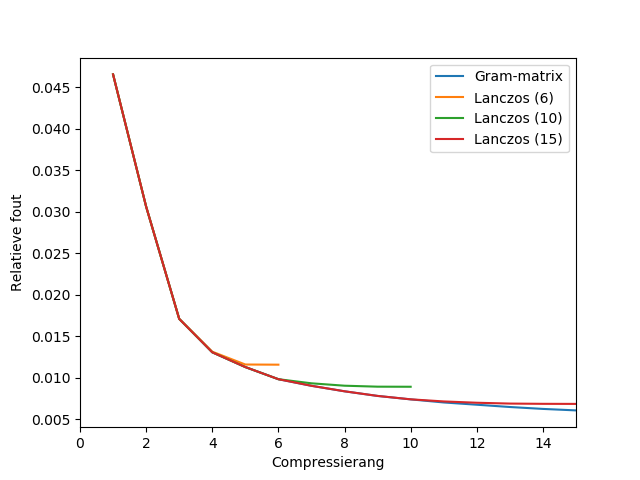
\includegraphics[scale=0.8]{images/lanczos_rank_comparison.png}
  \caption{Relatieve fout voor verschillende compressierangen en methoden bij het comprimeren van de eerste mode (de spectrale mode) van Cuprite. De getallen in de legende geven aan hoeveel Lanczos-iteraties uitgevoerd werden. Men ziet dat het nuttig kan zijn om meer iteraties uit te voeren dan de uiteindelijke compressierang.}
\label{fig:lanczos-rank-comparison}
\end{figure}

\subsubsection{Randomized SVD}

Wanneer we een afgeknotte SVD zoeken van een matrix $A \in \mathbb{R}^{m \times n}$ met $m \ll n$, zijn we eigenlijk ge\"interesseerd in de belangrijkste linker-singuliere vectoren, of met andere woorden, de beste basisvectoren om de verzameling kolomvectoren van $A$ in voor te stellen. Het is echter logisch dat vaak slechts een kleine deelverzameling van de kolomvectoren van $A$ al representatief is voor de volledige populatie en tot een even goede basis leidt. Op deze manier kan men de rekentijd van de SVD verkleinen zonder een grote fout te introduceren. Deze techniek wordt de \textit{randomized SVD} \cite{ref:randomized_svd} genoemd en wordt voor veel toepassingen gebruikt om de SVD te versnellen.\\

Concreet construeren we bij deze methode dus een matrix met een willekeurige verzameling kolommen van $A$ en berekenen we van deze steekproefmatrix de SVD om zo (de eerste kolommen van) $U$ te benaderen. De $\Sigma$ die hierbij berekend wordt is weliswaar niet accuraat, aangezien deze slechts het aandeel van de singuliere vectoren in de steekproef voorstelt, maar dit kan makkelijk gecorrigeerd worden door deze te vermenigvuldigen met $\sqrt{\frac{\text{populatiegrootte}}{\text{steekproefgrootte}}}$. Hierdoor wordt $\Sigma$ ook goed benaderd en kan deze gebruikt worden om bijvoorbeeld de compressierang te bepalen.\\

Verder kan de de SVD van de steekproefmatrix ook berekend worden met de bovenstaande methoden, om zo een grotere versnelling te bekomen.\\

\begin{table}[]
\centering
\begin{tabular}{|l|l|l|}
\hline
Methode & Gram-matrix & Steekproef + Gram-matrix\\ \hhline{|=|=|=|}
\input{data/randomized-svd-cuprite-test.tex}
\end{tabular}
\caption{Vergelijking tussen een typische uitvoering van de methode met de Gram-matrix met en zonder steekproef voor Cuprite met relatieve doelfout 0.025.}
\label{table:randomized-svd-cuprite-test}
\end{table}

In tabel \ref{table:randomized-svd-cuprite-test} vindt men een typische uitvoering met en zonder steekproef. Als steekproefgrootte per mode nemen we simpelweg 5 keer de originele rang. Merk op dat dit over slechts \'e\'en experiment gaat en men dus best geen conclusies trekt over bijvoorbeeld de absolute uitvoeringstijd. Wel kan men zien dat onze benaderingsmethode voor $\Sigma$ adequate precisie geeft. Verder geeft het gebruik van een steekproef in mode 2 een significante versnelling, terwijl in de andere modes de populatie te klein was ten opzichte van de originele rang om een steekproef te nemen. Uiteindelijk is er geen significante fout ge\"introduceerd door het gebruik van de steekproef.\\

\begin{table}[]
\centering
\begin{tabular}{|l|l|l|}
\hline
Methode & Gram-matrix & Steekproef + Gram-matrix\\ \hline
\input{data/randomized-svd-cuprite-average.tex}
\end{tabular}
\caption{Vergelijking tussen de methode met de Gram-matrix met en zonder steekproef voor Cuprite met relatieve doelfout 0.025 (10 experimenten).}
\label{table:randomized-svd-cuprite-average}
\end{table}

\begin{table}[]
\centering
\begin{tabular}{|l|l|l|}
\hline
Methode & Gram-matrix & Steekproef + Gram-matrix\\ \hline
\input{data/randomized-svd-mauna-kea-average.tex}
\end{tabular}
\caption{Vergelijking tussen de methode met de Gram-matrix met en zonder steekproef voor Mauna Kea met relatieve doelfout 0.025 (10 experimenten).}
\label{table:randomized-svd-mauna-kea-average}
\end{table}

We zien in tabel \ref{table:randomized-svd-cuprite-average} dat, voor deze dataset, de randomized SVD een degelijke versnelling geeft zonder een significant verschil in de fout of compressiefactor. Daarnaast is de variantie op de fout en compressiefactor erg klein. Bovendien toont tabel \ref{table:randomized-svd-mauna-kea-average} aan dat deze techniek ook goed werkt voor voor Mauna Kea, al is het met een steekproef van 20 keer de originele rang.\\

Verder hebben we als kleine optimizatie getest of het sorteren van de steekproefindices voor het selecteren van deze kolommen uit de steekproefmatrix effect heeft op de uitvoeringstijd. Dit kost rekenwerk maar kan eventueel een versnelling geven bij het kopi\"eren van de kolommen vanwege het betere \textit{memory access pattern}. In de praktijk bleef de rekentijd ongeveer hetzelfde, dus we gebruiken deze techniek verder niet.\\

\begin{figure}[]
  \centering
  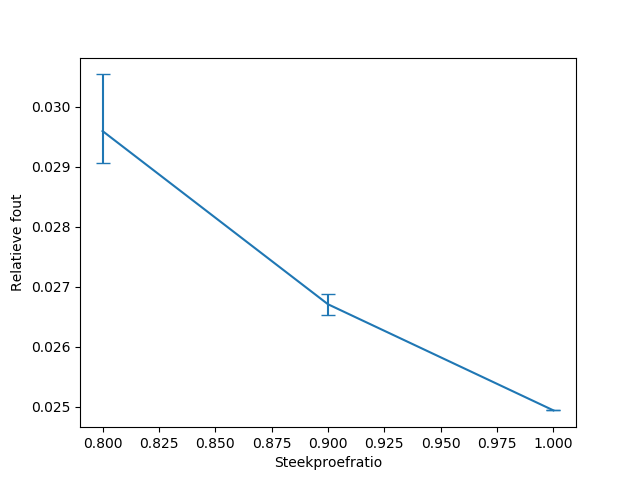
\includegraphics[scale=0.8]{images/randomized_svd_pavia_ratios.png}
  \caption{Compressiefout bij verschillende steekproefratios voor Pavia Centra met relatieve doelfout 0.025 (uitgemiddeld over 3 experimenten). De foutbalkjes stellen de minimale en maximale waarden voor over de verschillende experimenten.}
\label{fig:randomized-svd-pavia-ratios}
\end{figure}

In figuur \ref{fig:randomized-svd-pavia-ratios} ziet men echter dat de randomized SVD geen goede resultaten geeft bij Pavia Centre. Hierbij moesten we de steekproefratio (de verhouding tussen de steekproefgrootte en populatiegrootte) verhogen tot 1 om geen merkbare fout toe te voegen, maar in tabel \ref{table:randomized-svd-pavia-test} zien we dat een steekproefratio van 0.2 nog redelijk lijkt te werken voor de spectrale mode, de best comprimeerbare mode. Daarnaast zijn alle modes van Pavia significant slechter comprimeerbaar dan die van Cuprite. Hierdoor denken we dat de steekproefgrootte best groter gekozen wordt wanneer de mode slecht comprimeerbaar is.\\

De meest logische manier om de ``comprimeerbaarheid'' van een mode in te schatten, is echter door te kijken naar de verdeling van de singuliere waarden, die men pas kent na het berekenen van de SVD. Het lijkt ons dus moeilijk om voor een brede verzameling datasets op consistente wijze snel een goede steekproefgrootte te kiezen zonder verdere gegevens over de data, hoewel dit mogelijk verder onderzocht kan worden. Om deze reden zullen we de randomized SVD verder niet gebruiken, hoewel ze voor bepaalde datasets zeker een mooie versnelling kan opleveren.

\subsubsection{Besluit}

Na de resultaten van alle bovenstaande methodes te vergelijken, kiezen we ervoor om vanaf nu de methode met de Gram-matrix zonder verdere toevoegingen te gebruiken voor het berekenen van de SVD. Dit lijkt ons de snelste methode die geen significant effect heeft op de compressiefout- of factor.

\begin{table}[H]
\centering
\begin{tabular}{|l|l|l|}
\hline
Methode & Gram-matrix & Steekproef + Gram-matrix\\ \hhline{|=|=|=|}
\input{data/randomized-svd-pavia-test.tex}
\end{tabular}
\caption{Vergelijking tussen een uitvoering van de methode met de Gram-matrix met en zonder steekproef voor Pavia Centre met relatieve doelfout 0.025.}
\label{table:randomized-svd-pavia-test}
\end{table}
\section{Orthogonaliteitscompressie}

Men zou kunnen denken dat bij de Tuckerdecompositie de meeste ruimte ingenomen wordt door de kerntensor. Wanneer men namelijk naar tensoren met $k$ modes kijkt, waarbij de lengte per mode $n$ constant blijft en telkens gecomprimeerd wordt naar constante rang $r$, dan groeit de gecomprimeerde kerntensor met $O(r^k)$ en de factormatrices slechts met $O(knr)$, dus met $n, r$ constant en groeiende $k$ worden de factormatrices verwaarloosbaar.\\

In de praktijk werken we echter met een beperkt aantal modes en vaak lage compressierangen. Zelfs als we later reshapen verhogen we hiermeee $k$, maar verlagen we $n$ en $r$, dus het aandeel van de kerntensor zal hierdoor niet zozeer veel verhogen. Bijvoorbeeld, wanneer men de ST-HOSVD toepast op Cuprite met relatieve doelfout 0.025, comprimeert men van rang (512, 614, 190) naar (139, 192, 4) en nemen de factormatrices 64\% van het geheugen in. Bij Mauna Kea, een veel grotere dataset, is dit percentage 55\%. We kunnen dus concluderen dat het zeker interessant is om te kijken naar specifieke compressietechnieken voor de factormatrices.\\

We weten dat de factormatrices orthogonaal zijn en dit kunnen we benutten. Stel namelijk, we hebben een factormatrix $U \in \mathbb{R}^{n \times r}$ en verdelen deze op de volgende wijze:
\[
U = \begin{bmatrix}
A & c & \dots \\
B & x & \dots \\
\end{bmatrix}
\]
met $A \in \mathbb{R}^{(n-k) \times k}$, $B \in \mathbb{R}^{k \times k}$, $c \in \mathbb{R}^{n-k}$, $x \in \mathbb{R}^{k}$, voor willekeurige $1 \leq k < n$. Vanwege orthogonaliteit weten we dat:
\begin{align*}
\begin{bmatrix}
A \\
B \\
\end{bmatrix}^T
\begin{bmatrix}
c \\
x \\
\end{bmatrix}
&= 0 \\
A^T c + B^T x &= 0 \\
B^T x &= -A^T c
\end{align*}
Bijgevolg kunnen we $x$ berekenen als de oplossing van een lineair stelsel met $k$ onafhankelijke vergelijkingen en $k$ variabelen en moeten deze waarden niet opgeslagen worden. Theoretisch gezien kan men dus, door dit proces sequentieel uit te voeren voor $k = 1, \dots, n - 1$, een hele driehoek van $r (r - 1)/2$ elementen uit de matrix laten vallen. Om terug te komen op de eerdere voorbeelden: dit zou bij Cuprite en Mauna Kea neerkomen op 9.4\% en 7.5\% van alle waarden (inclusief kerntensor) respectievelijk. Men kan ook kiezen om de kolommen in een andere volgorde te verwerken, maar dit leek ons het beste zodat de herberekende waarden vooral zitten in de latere singuliere vectoren, die minder belangrijk zijn.
\section{Quantisatie}
\label{sec:quantisatie}

Tot nu toe hebben we altijd gewerkt met 32-bit floating-point getallen, wat voor onze doeleinden genoeg rekenprecisie geeft. Wanneer we deze getallen echter willen opslaan, zouden we ze liefst compacter willen voorstellen. Dit gaan we doen door te quantiseren: hierbij ronden we elke waarde af naar de dichtsbijzijnde waarde uit een beperkte verzameling die we zelf defini\"eren. Deze afronding zal de uiteindelijke fout op het eindresultaat verhogen, maar door deze verzamelingen goed te kiezen zullen we proberen een optimale afweging tussen de compressiefout en -factor te bekomen.\\

Wanneer we in deze sectie spreken over ``quantiseren naar $b$ bits'', doen we dit door de originele waarden te verschuiven en te schalen met specifieke waarden (die mee opgeslagen worden als 32-bit floats), zodat het nieuwe bereik exact overeenkomt met $[0, 2^b - 1]$. Hierna bekomen we de gequantiseerde waarden door alle waarden af te ronden naar het dichtsbijzijnde gehele getal. Dit is niet de enige mogelijke transformatie, maar we zullen ons in deze tekst hiertoe beperken. Verder zullen we de compressiefactor meten door telkens te quantiseren naar een verzameling met grootte gelijk aan $2^b$ (niet zozeer altijd met dezelfde $b$), waarna de geheugenruimte van per waarde geteld wordt als $b$ bits. 

\subsection{Kerntensor}

We zullen pas in de volgende subsectie quantisatietechnieken voor de factormatrices bespreken, maar zullen toch voor de komende experimenten moeten kiezen hoe deze verwerkt worden om de fout op het eindresultaat te berekenen. Zoals we in de vorige sectie zagen, wordt er quasi geen fout toegevoegd door de factormatrices te quantiseren naar 16 bits (en $\tau$ niet te quantiseren), dus we zullen dit ook doen voor de rest van de deze subsectie.

\subsubsection{Structuur van de kerntensor}

We weten dat gedurende de ST-HOSVD, bij het berekenen van de co\"ordinaten in de nieuwe basis, de eerste basisvectoren belangrijker zijn. Hierdoor zullen de absolute waarden van de eerste co\"ordinaten typisch ook groter zijn. Door dit proces meerdere malen toe te passen terwijl men over de modes itereert, zal men in feite de ``energie'' van de tensor concentreren in de posities met lage indices. De waarden in de uiteindelijke kerntensor zullen dus niet uniform verdeeld zijn.\\

Om hiermee rekening te houden zullen we in de rest van deze subsectie werken met ``lagen''. Met laag $i$ van een tensor bedoelen we de verzameling van posities met alle indices kleiner dan of gelijk aan $i$ en minstens \'e\'en index gelijk aan $i$ (denk aan schillen). In figuur \ref{fig:core-tensor-layers} wordt dit ge\"illustreerd. In de praktijk is de ongelijkheid tussen de lagen erg groot (zie figuur \ref{fig:core-tensor-values-distribution}, let op de logaritmische schaal).\\

\begin{figure}[H]
  \centering
  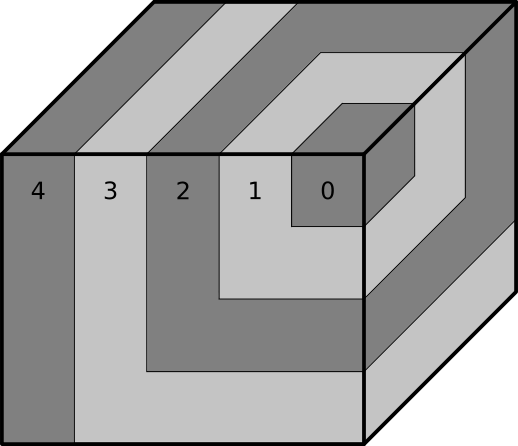
\includegraphics[scale=0.7]{images/core_tensor_layers.png}
  \caption{Lagen 0, \dots, 4 in een $5 \times 4 \times 3$ tensor.}
\label{fig:core-tensor-layers}
\end{figure}
\begin{figure}[H]
  \centering
  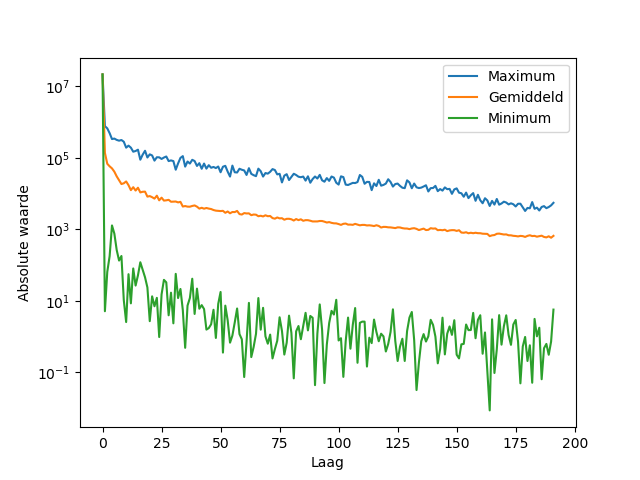
\includegraphics[scale=0.7]{images/core_tensor_values_distribution.png}
  \caption{Verdeling van absolute waarden in kerntensor bij Cuprite met relatieve doelfout 0.025.}
\label{fig:core-tensor-values-distribution}
\end{figure}

\newpage
Aangezien de meeste informatie in de eerste lagen zit, zullen we deze ongequantiseerd opslaan als 32-bit floats. Figuur \ref{fig:core-tensor-unquantized-portion} toont het effect van het aantal ongequantiseerde lagen bij vari\"erende aantallen quantisatiebits. Als quantisatietechniek gebruiken we simpelweg globale quantisatie: alle waarden buiten de eerste lagen worden gequantiseerd met hetzelfde aantal bits. Men ziet dat al een klein aantal lagen niet quantiseren een groot effect heeft op de fout met een insignificant effect op de compressiefactor. We kiezen ervoor om in het algemeen het aantal ongequantiseerde lagen zo te kiezen dat de norm van deze waarden minstens gelijk is aan 99.5\% van de norm van de tensor, wat bij Cuprite met relatieve doelfout 0.025 neerkomt op slechts 2 lagen.

\begin{figure}[H]
  \centering
  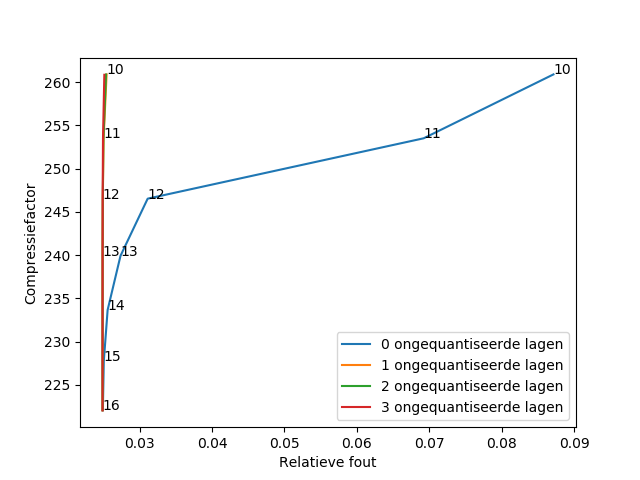
\includegraphics[scale=0.7]{images/core_tensor_unquantized_portion.png}
  \caption{Relatieve fout versus compressiefactor bij Cuprite met relatieve doelfout 0.025. De labels geven het aantal quantisatiebits aan.}
\label{fig:core-tensor-unquantized-portion}
\end{figure}

\subsubsection{Gelaagde quantisatie met constant aantal bits}

Zoals we eerder in figuur \ref{fig:core-tensor-values-distribution} zagen, zijn de waarden binnen de kerntensor erg ongelijk verdeeld, zelfs na het wegfilteren van de eerste twee lagen. Het is dus erg verspillend om alle andere waarden te quantiseren met hetzelfde aantal bits en dezelfde quantisatiestap, want het bereik van de waarden zal gedomineerd worden door het bereik van de eerste lagen, terwijl de laatste lagen slechts een erg klein deel van dit spectrum gebruiken.\\

Om dit op te lossen kunnen we elke laag apart quantiseren met een vast aantal bits dat constant blijft over de hele tensor, waardoor het bereik mooi past voor elke laag. Hierbij moeten we wel metadata gaan opslaan per laag en aangezien deze groeit met de afmetingen van de tensor zullen we deze meetellen in het geheugengebruik. Echter, bij een effici\"ente implementatie komt dit slechts neer op 12 bytes per laag, dus de \textit{overhead} van deze techniek is erg beperkt.

\subsubsection{Gelaagde quantisatie met variabel aantal bits}

Door het aantal quantisatiebits constant te houden over verschillende lagen, zal de quantisatiestap fijner worden voor de latere lagen. We weten echter dat alle kolommen uit de factormatrices genormaliseerd zijn, dus een vaste absolute fout op een waarde in de kerntensor zal zich onafhankelijk van de positie van deze waarde vertalen naar ongeveer dezelfde fout op het eindresultaat. Het is dus logischer om de latere lagen te quantiseren met een even grote stap, waardoor we minder bits nodig hebben.\\

Bij deze techniek zullen we voor elke laag een nieuw aantal quantisatiebits kiezen. We minimaliseren dit aantal zodat de quantisatiestap voor deze laag onder een bepaalde maximale stapgrootte ligt. We zullen deze controleren door expliciet het aantal quantisatiebits voor de eerste ongequantiseerde laag (de bits-parameter) te kiezen en dan de resulterende quantisatiestap gebruiken als bovengrens voor de verdere lagen. Voor het opslaan van het gekozen aantal bits zullen we \'e\'en byte extra per laag tellen, maar dit heeft natuurlijk geen significant effect.

\begin{figure}[H]
  \centering
  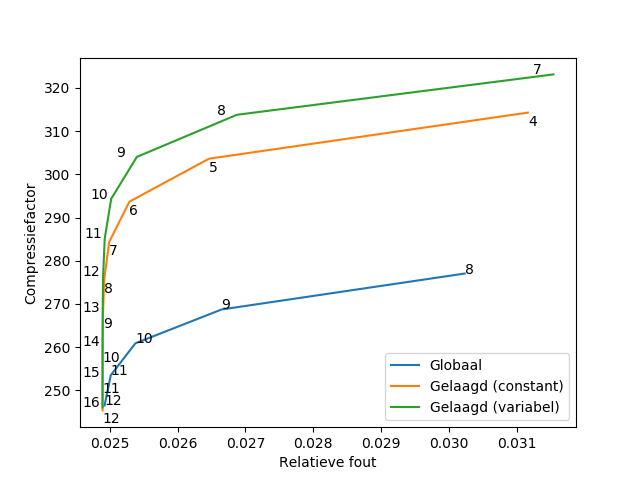
\includegraphics[scale=0.7]{images/core_tensor_quantization_comparison.png}
  \caption{Relatieve fout versus compressiefactor bij Cuprite met relatieve doelfout 0.025 en verschillende quantisatiemethoden voor de kerntensor. De labels geven de bits-parameterwaarden aan.}
\label{fig:core-tensor-quantization-comparison}
\end{figure}

\subsubsection{Besluit}

We hebben drie mogelijke quantisatietechnieken voor de kerntensor besproken: globale quantisatie en gelaagde quantisatie met een constant of variabel aantal bits. In figuur \ref{fig:core-tensor-quantization-comparison} zien we een experimentele vergelijking. Zoals verwacht comprimeert globale quantisatie het slechtste en kan men de gelaagde quantisatie verbeteren door te werken met een variabel aantal bits. Omwille van dit resultaat zullen we vanaf nu deze laatste techniek gebruiken (en specifiek voor de rest van deze sectie en sectie \ref{sec:encodering} met een bits-parameter van 12).

\subsection{Factormatrices}
\label{sec:quantisatie-factor-matrices}

Na de orthogonaliteitscompressie zal elke factormatrix voorgesteld worden als de combinatie van reflectoren en $\tau$-waarden (die samengevoegd worden tot \'e\'en $\tau$-vector per factormatrix). Zoals eerder besproken zullen we de $\tau$-vectoren niet quantiseren, omdat deze belangrijker zijn dan de andere waarden in de factormatrices en ons slechts 4 bytes per kolom per factormatrix kost. De waarden van de reflectoren nemen echter veel ruimte in en moeten best gequantiseerd worden.

\begin{figure}[H]
  \centering
  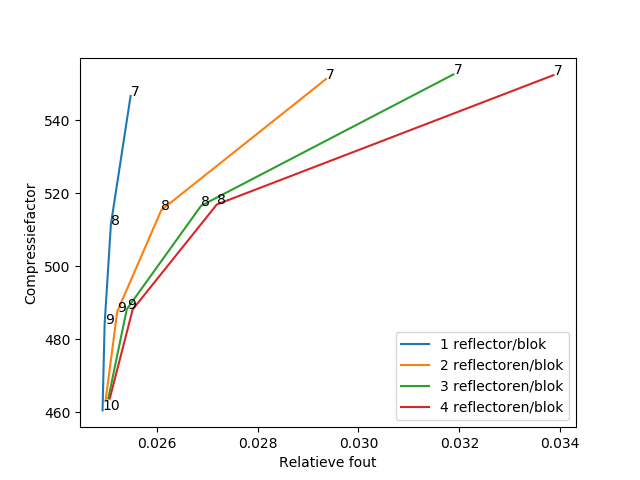
\includegraphics[scale=0.7]{images/factor_matrix_quantization_block_cols.png}
  \caption{Relatieve fout versus compressiefactor bij Cuprite met relatieve doelfout 0.025 en verschillende blokgroottes voor de quantisatie van de factormatrices. Quantisatie gebeurde gelaagd met norm-gebaseerde bit-aantal-selectie (zie vervolg subsectie). De labels geven de bits-parameterwaarden aan.}
\label{fig:factor-matrix-quantization-block-cols}
\end{figure}

Een eerste manier om dit te doen is weer met globale quantisatie per factormatrix (dus we berekenen \'e\'en specifiek bereik per matrix, niet voor alle matrices samen). We zagen echter al in de vorige subsectie dat het nuttig is om de waarden onder te verdelen in blokken, waardoor een specifieker bereik kan worden vastgelegd. Een gemiddelde reflector uit een factormatrix bevat echter veel minder waarden dan een gemiddelde laag uit de kerntensor, dus men zou kunnen proberen om meerdere reflectoren te groeperen per blok om zo de \textit{overhead} van de metadata (12 bytes per blok, eventueel 1 byte extra bij een variabel aantal bits) te beperken. Desalniettemin toont figuur \ref{fig:factor-matrix-quantization-block-cols} aan dat het beter is om dit niet te doen. We hebben ook ge\"experimenteerd met technieken om het aantal reflectoren per blok dynamisch te kiezen in functie van de dimensie van de reflector en het aantal quantisatiebits, maar dit gaf hetzelfde resultaat.\\

Om het aantal quantisatiebits te selecteren, kunnen we ook verschillende methoden gebruiken. De simpelste optie is om de bits-parameter te gebruiken als het constante aantal quantisatiebits voor elke reflector, maar hierbij houdt men geen rekening met enkele aspecten:

\begin{enumerate}

\item De eerste reflector be\"invloedt de reconstructie van alle kolommen van de factormatrix, de tweede reflector be\"invloedt alle kolommen buiten de eerste, ... Bijgevolg zijn de eerste reflectoren belangrijker en zou men deze met meer precisie kunnen bijhouden. Aangezien dit effect moeilijk te quantiseren valt houden we hier geen rekening mee.

\item De eerste singuliere vectoren zijn belangrijker dan de laatste, waardoor we beter meer precisie gebruiken voor deze. Bij ``norm-gebaseerde'' selectie zullen we het aantal bits per waarde binnen een reflector ongeveer proportioneel kiezen met het logaritme van de norm van de corresponderende snede uit de kerntensor (de waarden die later vermenigvuldigd zullen worden met corresponderende singuliere vector). De bits-parameter legt vast hoeveel quantisatiebits er voor de eerste reflector gekozen moeten worden.

\item De eerste reflectoren hebben een hogere dimensie en worden dus voorgesteld door meer waarden, waardoor het aantal bits per waarde hier misschien verlaagd moet worden. Bij ``norm- en dimensie-gebaseerde'' selectie zal het totaal aantal gebruikte bits per reflector ongeveer proportioneel zijn met de norm van de corresponderende snede uit de kerntensor. Zoals eerder wordt het aantal quantisatiebits per waarde voor de eerste reflector vastgelegd door de bits-parameter.

\end{enumerate}

In figuur \ref{fig:factor-matrix-quantization-comparison} vindt men een vergelijking van de besproken methoden. Zoals verwacht is gelaagde quantisatie opnieuw veel beter. Voor de bitselectie is de norm-gebaseerde techniek het beste, gevolgd door de norm- en dimensie-gebaseerde techniek en uiteindelijk constante selectie. Men zou dit kunnen verklaren door het effect van het eerste aspect dat we eerder bespraken (omzetting van reflectoren naar singuliere vectoren). Dit hebben we namelijk niet in rekening gebracht maar zou de norm-gebaseerde selectie moeten helpen. In ieder geval is dit de beste techniek en zal deze vanaf nu gebruikt worden. Voor de volgende sectie zullen we werken met een bits-parameter van 10, waardoor er geen merkbare fout toegevoegd zal worden.

\begin{figure}[H]
  \centering
  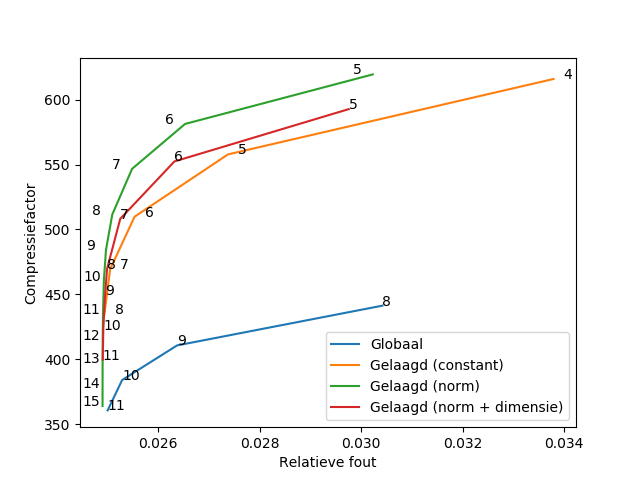
\includegraphics[scale=0.6]{images/factor_matrix_quantization_comparison.png}
  \caption{Relatieve fout versus compressiefactor bij Cuprite met relatieve doelfout 0.025. De labels geven de bits-parameterwaarden aan.}
\label{fig:factor-matrix-quantization-comparison}
\end{figure}

\section{Afstellen van de parameters}
\chapter{Compressie na hervorming}
\label{hoofdstuk:hervorming}

Zoals we eerder aan het begin van sectie \ref{sec:orthogonaliteitscompressie} bespraken, nemen de factormatrices van de Tucker-decomposities van onze datasets een groot deel van de totale opslagruimte in. Voor hoog-dimensionale tensoren is dit effect echter kleiner en bestaat de compressie bijna volledig uit de kerntensor. Onze originele data is 3D, maar in dit hoofdstuk zullen we deze hervormen naar 5D en onderzoeken of we hiervoor effici\"entere compressie-algoritmes kunnen ontwikkelen.

\section{Hervormen van de datasets}

In dit hoofdstuk zullen we de originele datasets telkens omzetten van drie naar vijf modes. Dit gebeurt aan de hand van hervorming, wat simpelweg neerkomt op een herinterpretatie van het geheugen. Bijvoorbeeld, stel dat we een 1D-tensor hebben met 200 elementen. Men kan deze interpreteren als een tensor met vorm (200), maar ook als een 2D-tensor met vorm (10, 20). Als men het dan heeft over het element op positie $(i, j)$, komt dit neer op het element met index $20i + j$ (in het geval van de \textit{row-major}-conventie). Merk op dat de interne opslag van de tensor hiervoor niet aangepast moet worden, alleen de metadata.\\

Men kan deze operatie uitvoeren op een willekeurige verzameling modes van een tensor. Zo zullen we vanaf nu onze datasets hervormen door elke spatiale mode op te splitsen in twee nieuwe modes. Op deze manier zijn de afmetingen van alle modes redelijk klein, op de spectrale mode na, die sowieso al erg goed comprimeert. Ter illustratie, bij Mauna Kea komt dit neer op een hervorming van (2704, 729, 199) naar (52, 52, 27, 27, 199).\\

We zullen in dit hoofdstuk werken met datasets waarvan de spatiale modes afmetingen hebben die exact kwadraten zijn, zodat de initi\"ele mode van grootte $n^2$ kan opgesplitst worden in twee modes met grootte $n$. Op zich zijn andere factorizaties ook mogelijk, maar om praktische redenen beperken we ons in ons onderzoek tot kwadratische afmetingen. Mauna Kea en Pavia Centre voldoen al aan deze beperking. Indian Pines en Cuprite niet, dus we zullen deze datasets voor de komende hoofdstukken vervangen door versies waarbij alleen de pixels met de laagste indices uitgeknipt worden. Hierbij ronden we de afmeting van elke spatiale mode af naar het dichtsbijzijnde kleinere kwadraat.

\section{Tucker-decompositie met hervorming}

Als eerste compressiemethode kunnen we simpelweg de ST-HOSVD berekenen van de hervormde tensor. In figuur \ref{fig:reshaped_tucker_st_hosvd_results} kan men de afweging zien tussen compressiefout en -factor voor verschillende datasets, zonder (blauw) en met (oranje) het hervormen van de data. Alleen de ST-HOSVD werd uitgevoerd, zonder orthogonaliteitscompressie (dit helpt sowieso al minder in het geval met hervorming, aangezien de factormatrices kleiner zijn), quantisatie of encodering. We zien dat na deze eerste compressiefase de Tucker-decompositie even goed tot significant slechter scoort afhankelijk van de dataset en gewenste fout. Om deze reden zullen we de Tucker-decompositie met hervorming niet verder onderzoeken.

\begin{figure}[H]
\centering
\begin{subfigure}{0.48\textwidth}
  \centering
  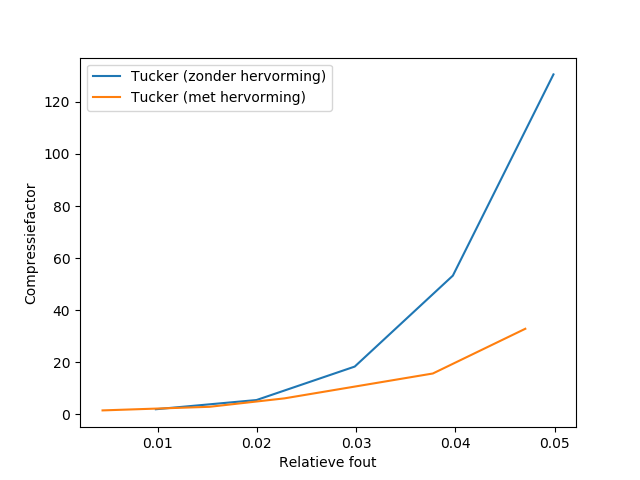
\includegraphics[width=\linewidth]{images/reshaped_tucker_st_hosvd_results_Indian_Pines.png}
  \caption{Indian Pines}
\end{subfigure}
\begin{subfigure}{0.48\textwidth}
  \centering
  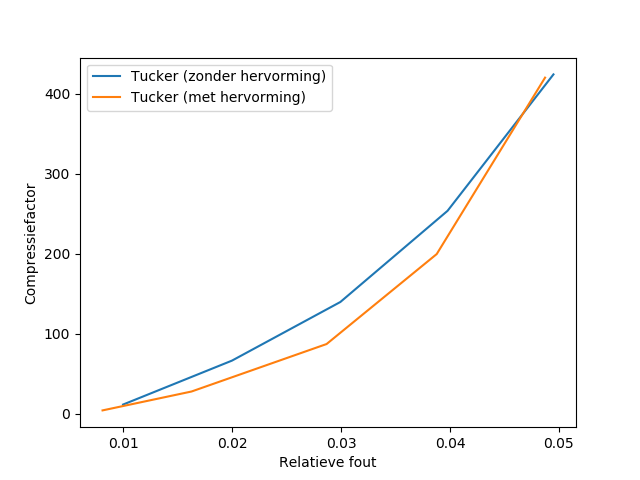
\includegraphics[width=\linewidth]{images/reshaped_tucker_st_hosvd_results_Cuprite.png}
  \caption{Cuprite}
\end{subfigure}
\\
\begin{subfigure}{0.48\textwidth}
  \centering
  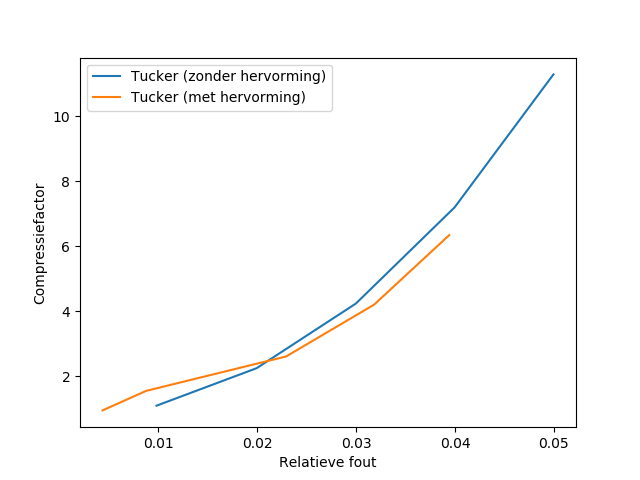
\includegraphics[width=\linewidth]{images/reshaped_tucker_st_hosvd_results_Pavia_Centre.png}
  \caption{Pavia Centre}
\end{subfigure}
\begin{subfigure}{0.48\textwidth}
  \centering
  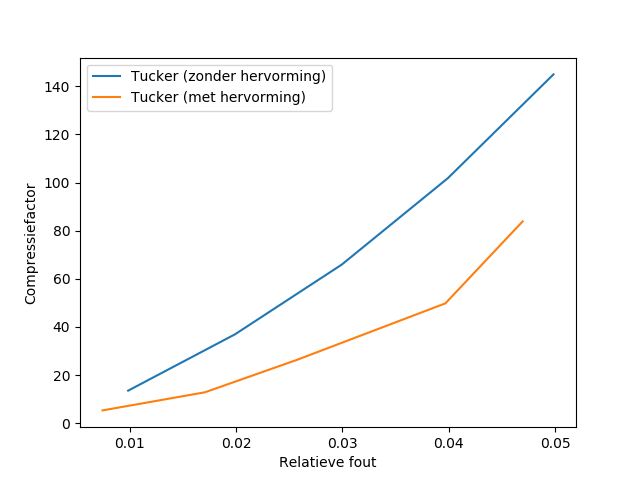
\includegraphics[width=\linewidth]{images/reshaped_tucker_st_hosvd_results_Mauna_Kea.png}
  \caption{Mauna Kea}
\end{subfigure}
\caption{Resultaten van de Tucker-decompositie zonder (blauw) en met (oranje) hervorming voor verschillende datasets, na alleen het uitvoeren van de ST-HOSVD (dus zonder orthogonaliteitscompressie, quantisatie of encodering).}
\label{fig:reshaped_tucker_st_hosvd_results}
\end{figure}

\section{Tensor trains}

Naast de Tucker-decompositie bestaan er ook andere tensordecomposities, zoals \textit{tensor trains} \cite{ref:tensor_trains}. Deze decompositie is specifiek nuttig voor het comprimeren van hoog-dimensionale tensoren, waardoor ze interessant is om te onderzoeken in dit hoofdstuk.

\subsection{De decompositie}

Ter herinnering: bij een Tucker-decompositie benaderen we een tensor $A \in \mathbb{R}^{n_1 \times n_2 \times \dots \times n_d}$ door een kerntensor $B \in \mathbb{R}^{r_1 \times r_2 \times \dots \times r_d}$ en factormatrices $U_1 \in \mathbb{R}^{n_1 \times r_1}$, $U_2 \in \mathbb{R}^{n_2 \times r_2}$, $\dots$, $U_d \in \mathbb{R}^{n_d \times r_d}$. De reconstructie gebeurt dan als volgt:
\[
A \approx B \times_1 U_1 \times_2 U_2 \times_3 \dots \times_d U_d
\]
waarbij $C \times_n U_n$ het n-mode product is van de tensor $C$ en matrix $U_k$. Een tensor train is vrij analoog, maar voegt voor elke mode een hervormingsstap toe. Hierbij hebben we een kerntensor $B \in \mathbb{R}^{r_{d-1},n_d}$, factormatrices $U_1 \in \mathbb{R}^{n_1 \times r_1}$, $U_2 \in \mathbb{R}^{r_1 n_2 \times r_2}$, $U_3 \in \mathbb{R}^{r_2 n_3 \times r_3}$, $\dots$, $U_{d-1} \in \mathbb{R}^{r_{d-2} n_{d-1} \times r_{d-1}}$ en de volgende formule:
\[
A \approx h(\dots h(h(B, r_{d-1} \times n_d) \times_1 U_{d-1}, r_{d-2} \times n_{d-1} \times n_d) \times_1 U_{d-2} \dots, r_1 \times n_2 \times \dots \times n_d) \times_1 U_1
\]
waarbij $h(C, \text{vorm})$ de hervormingsfunctie is die de tensor $C$ hervormt naar de gegeven vorm. Ter illustratie zullen we de constructieprocedure van een Tucker-decompositie vergelijken met die van een tensor train. Bij het uitvoeren van een normale ST-HOSVD op een 5D-tensor ($n_1 \times n_2 \times n_3 \times n_4 \times n_5$) ondergaat de kerntensor de volgende transformaties:

\begin{enumerate}
\item Comprimeer naar $r_1 \times n_2 \times n_3 \times n_4 \times n_5$
\item Comprimeer naar $r_1 \times r_2 \times n_3 \times n_4 \times n_5$
\item Comprimeer naar $r_1 \times r_2 \times r_3 \times n_4 \times n_5$
\item Comprimeer naar $r_1 \times r_2 \times r_3 \times r_4 \times n_5$
\item Comprimeer naar $r_1 \times r_2 \times r_3 \times r_4 \times r_5$
\end{enumerate}

Met kleine aanpassingen aan de ST-HOSVD kunnen we deze procedure even goed gebruiken om een tensor train te berekenen, waarbij de volgende stappen uitgevoerd worden:

\begin{enumerate}
\item Comprimeer naar $r_1 \times n_2 \times n_3 \times n_4 \times n_5$
\item Hervorm naar $r_1 n_2 \times n_3 \times n_4 \times n_5$
\item Comprimeer naar $r_2 \times n_3 \times n_4 \times n_5$
\item Hervorm naar $r_2 n_3 \times n_4 \times n_5$
\item Comprimeer naar $r_3 \times n_4 \times n_5$
\item Hervorm naar $r_3 n_4 \times n_5$
\item Comprimeer naar $r_4 \times n_5$
\item Hervorm naar $r_4 n_5$
\end{enumerate}

Elke iteratie, na de compressie, voegen we dus de twee eerste modes van de tensor samen, tot er slechts \'e\'en mode overblijft. Men zou kunnen redeneren dat, als men een $k$-D tensor van $n \times n \times \dots \times n$ comprimeert, telkens naar een compressierang $r$, de tensor train slechts $O(knr^2)$ ruimte inneemt. Er zijn namelijk $nr$ elementen in de eerste factormatrix, $nr^2$ elementen in elke andere factormatrix en $rn$ elementen in de uiteindelijke kerntensor. Bij de Tucker-decompositie is de ingenomen ruimte $O(r^k + knr)$, dus voor hoge $k$ zouden tensor trains het beter moeten doen. Deze redenering houdt echter geen rekening met het effect van telkens te comprimeren naar een vaste compressierang, wat een grote fout zou kunnen introduceren. Bijgevolg zullen we experimenteel moeten bepalen hoe effectief deze methode is in de praktijk.

\begin{figure}[H]
\centering
\begin{subfigure}{0.48\textwidth}
  \centering
  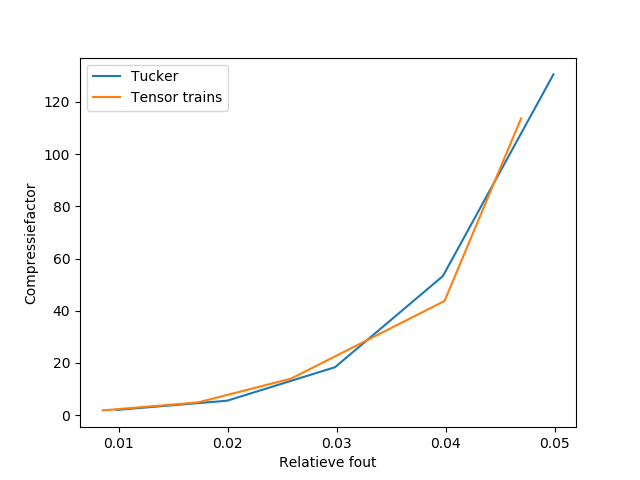
\includegraphics[width=\linewidth]{images/tensor_trains_st_hosvd_results_Indian_Pines.png}
  \caption{Indian Pines}
\end{subfigure}
\begin{subfigure}{0.48\textwidth}
  \centering
  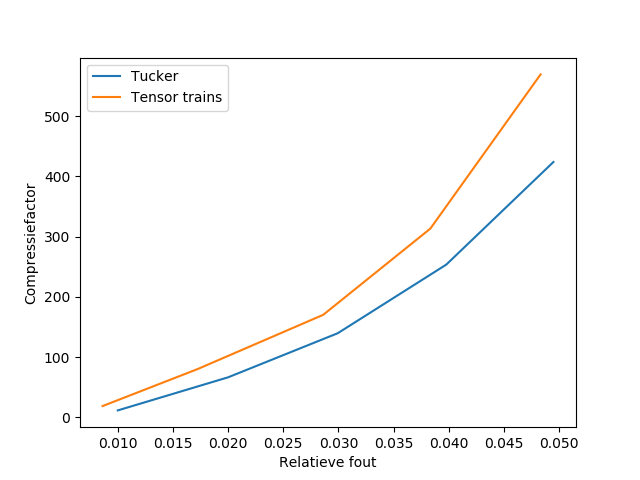
\includegraphics[width=\linewidth]{images/tensor_trains_st_hosvd_results_Cuprite.png}
  \caption{Cuprite}
\end{subfigure}
\\
\begin{subfigure}{0.48\textwidth}
  \centering
  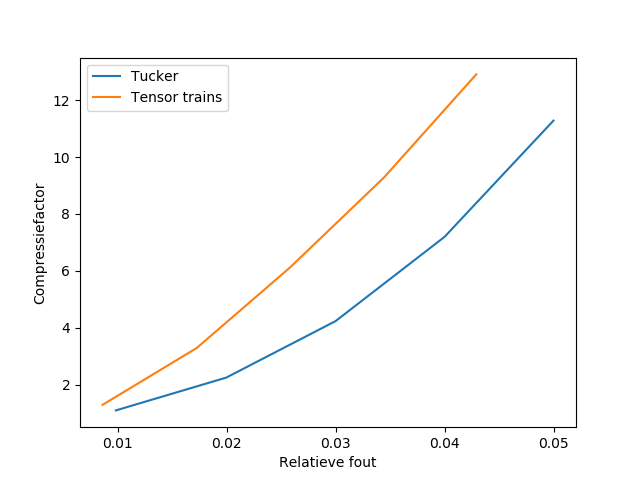
\includegraphics[width=\linewidth]{images/tensor_trains_st_hosvd_results_Pavia_Centre.png}
  \caption{Pavia Centre}
\end{subfigure}
\begin{subfigure}{0.48\textwidth}
  \centering
  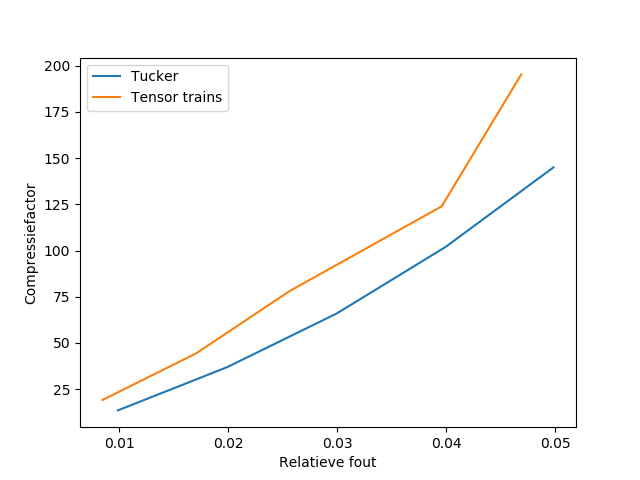
\includegraphics[width=\linewidth]{images/tensor_trains_st_hosvd_results_Mauna_Kea.png}
  \caption{Mauna Kea}
\end{subfigure}
\caption{Resultaten van de Tucker-decompositie (zonder hervorming, blauw) en tensor trains (oranje) voor verschillende datasets, na alleen het uitvoeren van de ST-HOSVD (dus zonder orthogonaliteitscompressie, quantisatie of encodering).}
\label{fig:tensor_trains_st_hosvd_results}
\end{figure}

\subsection{Eerste resultaten}

Analoog aan de vorige sectie, hebben we in figuur \ref{fig:tensor_trains_st_hosvd_results} de resultaten na alleen het uitvoeren van de ST-HOSVD vergeleken tussen tensor trains en de Tucker-decompositie (zonder hervorming). Bij Indian Pines, een kleine en minder belangrijke dataset, doen beide methoden het ongeveer even goed, terwijl in alle andere gevallen tensor trains betere resultaten geven. Het is dus zeker interessant om deze techniek verder te onderzoeken.

\subsection{Verdere uitwerking}

Zoals in hoofdstuk \ref{hoofdstuk:tucker} uitgebreid beschreven werd, moeten er bij het ontwikkelen van een volledig compressie-algoritme een aantal ontwerpkeuzes gemaakt worden. Aangezien we de meeste technieken hergebruiken, zullen we dit hier slechts kort bespreken:

\begin{enumerate}
\item \textbf{Versnellen van de ST-HOSVD:}
\begin{enumerate}
\item \textbf{Modevolgorde:} Zoals eerder, de spectrale mode wordt eerst verwerkt, gevolgd door de spatiale modes in volgorde van dalende grootte.
\item \textbf{Versnellen van de SVD:} De SVD wordt berekend aan de hand van de methode met Gram-matrix, zolang deze werkelijk kleiner is dan de originele matrix. Bij de latere modes kan $n_{i+1} n_{i+2} \dots n_k$, het aantal te verwerken vectoren, kleiner zijn dan de dimensie van deze vectoren $r_{i-1} n_i$. In deze gevallen zullen we de SVD op de normale manier berekenen.
\end{enumerate}
\item \textbf{Orthogonaliteitscompressie:} Zoals eerder gebruiken we de methode met Householder-reflecties, aangezien deze een ideaal resultaat geven.

\item \textbf{Quantisatie:}
\begin{enumerate}

\item \textbf{Kerntensor:} In figuur \ref{fig:tensor-trains-core-tensor-size} zien we dat de factormatrices bijna alle ruimte innemen bij een typische tensor train. Bijgevolg zullen we de kerntensor simpelweg niet quantiseren.

\begin{figure}[]
  \centering
  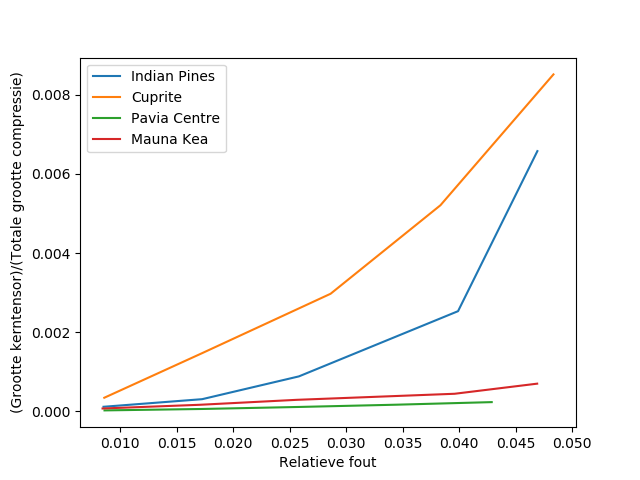
\includegraphics[scale=0.7]{images/tensor_trains_core_tensor_size.png}
  \caption{Het aandeel van de kerntensor in de compressie bij tensor trains, na alleen het uitvoeren van de ST-HOSVD.}
\label{fig:tensor-trains-core-tensor-size}
\end{figure}

\item \textbf{Factormatrices:} Zoals eerder, we gebruiken gelaagde quantisatie met norm-gebaseerde bit-aantal-selectie.
\end{enumerate}
\item \textbf{Encodering:} Zoals eerder, we zullen adaptieve encodering gebruiken zonder benaderende Huffman-codes.

\begin{figure}[]
  \centering
  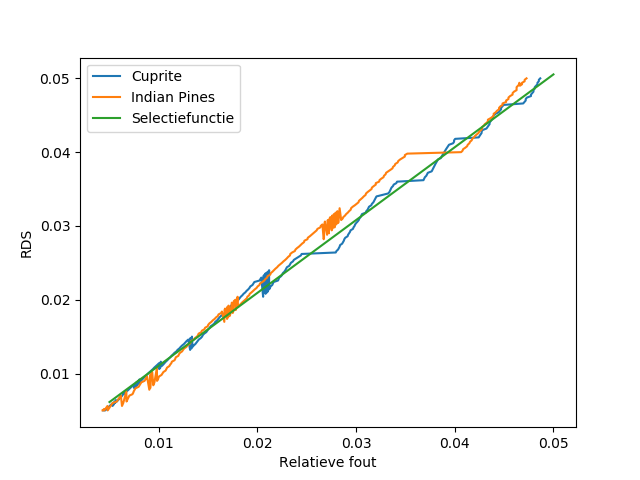
\includegraphics[scale=0.7]{images/filtered_sweep_points_tensor_trains_RDS.png}
  \caption{RDS-waarden van steekproefoptima en de RDS-selectiefunctie.}
\label{fig:filtered-sweep-points-tensor-trains-RDS}
\end{figure}

\begin{figure}[]
  \centering
  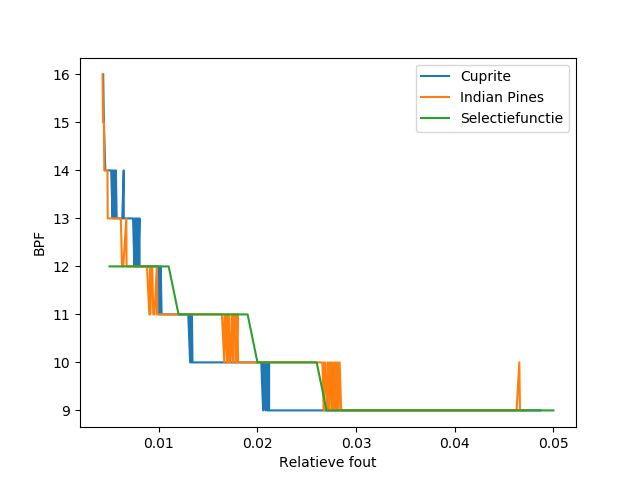
\includegraphics[scale=0.7]{images/filtered_sweep_points_tensor_trains_BPF.png}
  \caption{BPF-waarden van steekproefoptima en de BPF-selectiefunctie.}
\label{fig:filtered-sweep-points-tensor-trains-BPF}
\end{figure}

\item \textbf{Parameterselectie:} Aangezien de kerntensor niet meer gequantiseerd wordt, moeten alleen de RDS- en BPF-parameters afgesteld worden. Bij het verkennen van de parameterruimte beschouwen we de volgende domeinen: $RDS \in \{0.005, 0.0052, 0.0054, \dots, 0.05\}$ en $BPF \in \{16, 15, 14, \dots, 1\}$.
\begin{enumerate}

\item \textbf{Niet-adaptief:} Als we kijken naar de parameterwaarden die corresponderen met de steekproefoptima (Pareto-effici\"ente parametercombinaties), bekomen we figuren \ref{fig:filtered-sweep-points-tensor-trains-RDS} en \ref{fig:filtered-sweep-points-tensor-trains-BPF}. We kiezen de volgende selectiefuncties, op analoge wijze als in sectie \ref{sec:parameters}:
\begin{itemize}
\item $RDS = max(0.001, 0.986746*\text{kwaliteit} - 0.001199)$
\item $BPF = max(9, round(-132.505*\text{kwaliteit} + 13.048))$
\end{itemize}

\item \textbf{Adaptief:} We zullen, zoals eerder, ook een adaptieve selectieprocedure uitwerken. Hierbij wordt de RDS weer vast gekozen aan de hand van de RDS-selectiefunctie en verlagen we de BPF-waarde (startend bij de waarde gekozen door de BPF-selectiefunctie) totdat de compressiefout de kwaliteitsparameter overschrijdt. Omdat er maar \'e\'en parameter adaptief gekozen wordt in plaats van twee, is deze procedure veel simpeler dan bij Tucker-gebaseerde compressie.\\

In figuren \ref{fig:parameter_functions_results_including_adaptive_Cuprite_tensor_trains} en \ref{fig:parameter_functions_results_including_adaptive_Indian_Pines_tensor_trains} tonen we opnieuw een vergelijking van compressie met (niet-)adaptieve parameterselectie en met optimale parameters uit de steekproef van ons onderzoek. We zien dat er voor Cuprite en Indian Pines weinig verschil is tussen het adaptieve en niet-adaptieve resultaat. We hebben ook gekeken naar grotere datasets, maar daar werkte de niet-adaptieve methode ook even goed, zonder de extra rekenkost, dus we zullen niet verder werken met adaptieve parameterselectie voor tensor trains.

\end{enumerate}
\end{enumerate}

\newpage
\begin{figure}[H]
  \centering
  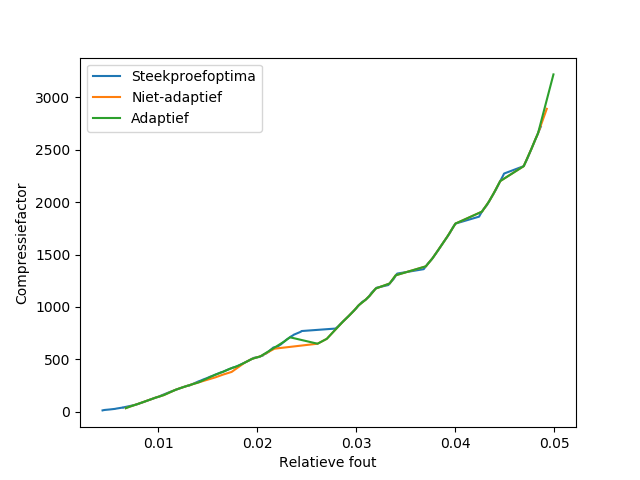
\includegraphics[scale=0.7]{images/parameter_functions_results_including_adaptive_Cuprite_tensor_trains.png}
  \caption{Resultaten van compressie met en zonder adaptieve parameterselectie voor Cuprite.}
  \label{fig:parameter_functions_results_including_adaptive_Cuprite_tensor_trains}
\end{figure}

\begin{figure}[H]
  \centering
  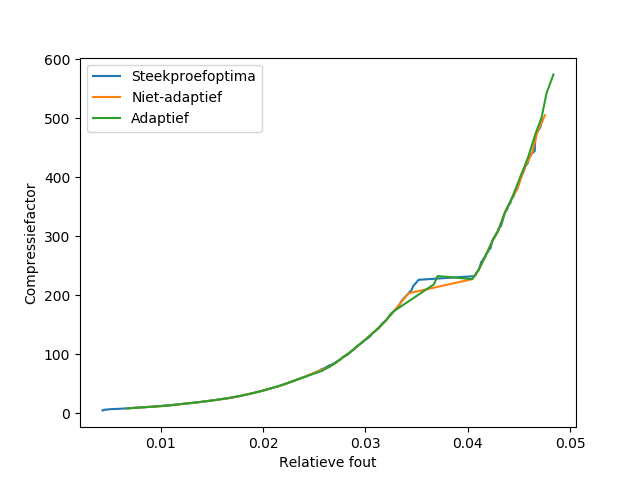
\includegraphics[scale=0.7]{images/parameter_functions_results_including_adaptive_Indian_Pines_tensor_trains.png}
  \caption{Resultaten van compressie met en zonder adaptieve parameterselectie voor Indian Pines.}
  \label{fig:parameter_functions_results_including_adaptive_Indian_Pines_tensor_trains}
\end{figure}

\newpage

\chapter{Resultaten}
\label{hoofdstuk:resultaten}

Na het ontwikkelen van zowel Tucker-gebaseerde als tensor-train-gebaseerde compressie-algoritmen, is het tijd om de uiteindelijke resultaten te bekijken. In dit hoofdstuk vergelijken we onze eigen compressietechnieken zowel met elkaar, met andere algemene methoden, zoals JPEG of videocompressie, als met een methode uit de literatuur. We sluiten nog af met enkele voorbeelden van gecomprimeerde hyperspectrale afbeeldingen.

\section{Tucker versus tensor trains}

In figuren \ref{fig:tucker-vs-tensor-trains-indian-pines}, \ref{fig:tucker-vs-tensor-trains-cuprite}, \ref{fig:tucker-vs-tensor-trains-pavia-centre} en \ref{fig:tucker-vs-tensor-trains-mauna-kea} tonen we de resultaten van Tucker-gebaseerde compressie en tensor-train-gebaseerde compressie voor verschillende datasets met vari\"erende kwaliteitsparameter. Zoals eerder besproken, wordt adaptieve parameterselectie alleen gebruikt bij de Tucker-methode bij kleine datasets (Indian Pines en Cuprite). We zien dat de tensor trains het altijd minstens even goed doen als Tucker zonder adaptieve parameterselectie en dat Tucker met adaptieve parameterselectie alleen beter scoort bij Indian Pines, een kleine en minder belangrijke dataset.\\

Bovendien zien we in figuur \ref{fig:tucker-vs-tensor-trains-times} dat de methode met tensor trains minstens even snel is als niet-adaptieve Tucker en zelfs significant sneller voor grote datasets. Om deze redenen lijken tensor trains ons over het algemeen beter en zullen we hierop de focus leggen in de volgende secties.

\begin{figure}[]
  \centering
  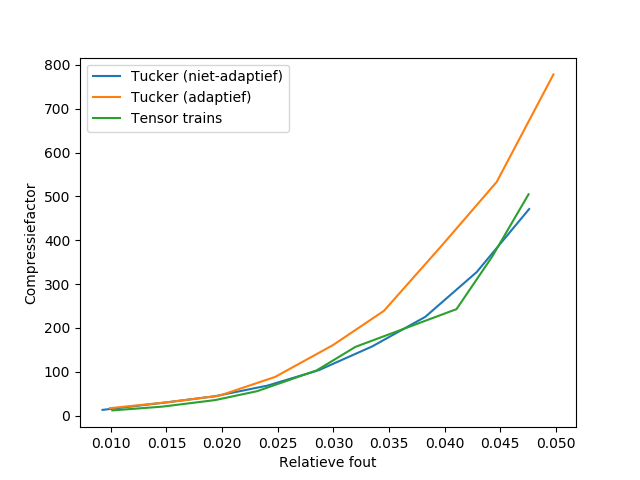
\includegraphics[scale=0.7]{images/tucker_vs_tensor_trains_Indian_Pines.png}
  \caption{Vergelijking tussen Tucker-gebaseerde compressie en tensor-train-compressie voor Indian Pines.}
\label{fig:tucker-vs-tensor-trains-indian-pines}
\end{figure}

\begin{figure}[]
  \centering
  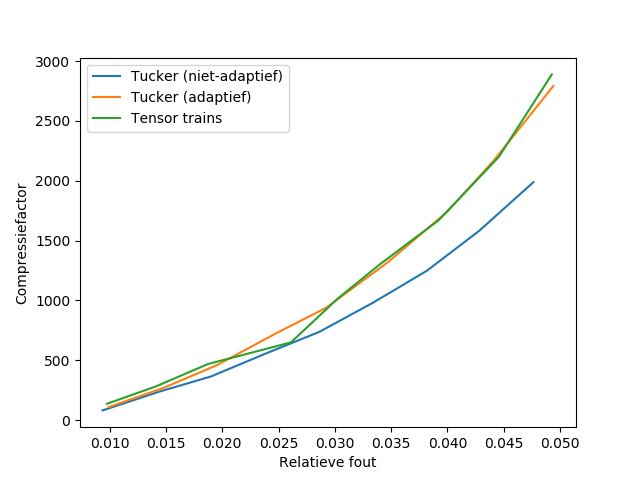
\includegraphics[scale=0.7]{images/tucker_vs_tensor_trains_Cuprite.png}
  \caption{Vergelijking tussen Tucker-gebaseerde compressie en tensor-train-compressie voor Cuprite.}
\label{fig:tucker-vs-tensor-trains-cuprite}
\end{figure}

\begin{figure}[]
  \centering
  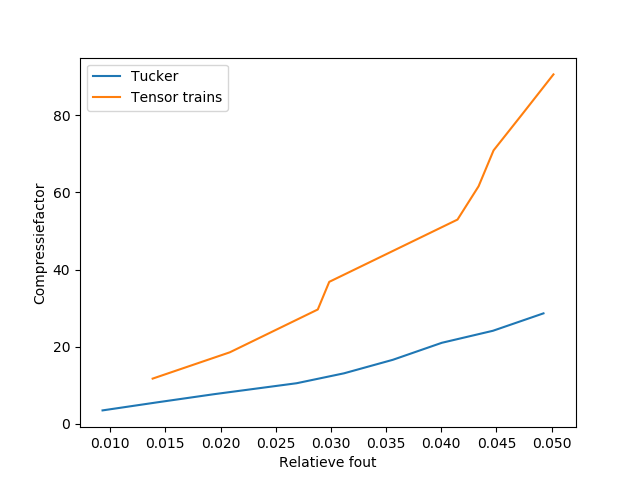
\includegraphics[scale=0.7]{images/tucker_vs_tensor_trains_Pavia_Centre.png}
  \caption{Vergelijking tussen Tucker-gebaseerde compressie en tensor-train-compressie voor Pavia Centre.}
\label{fig:tucker-vs-tensor-trains-pavia-centre}
\end{figure}

\begin{figure}[]
  \centering
  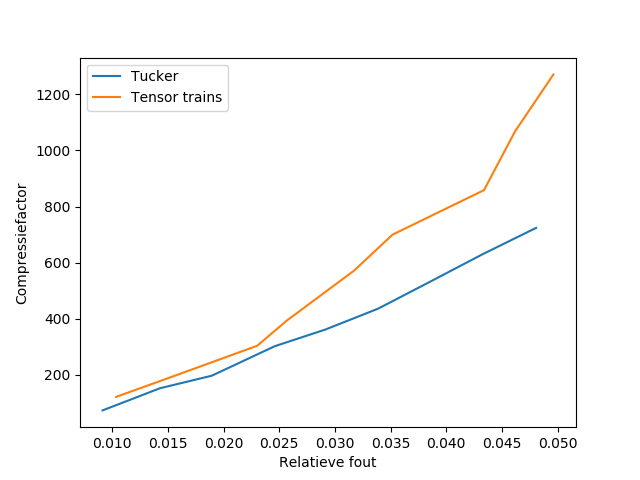
\includegraphics[scale=0.7]{images/tucker_vs_tensor_trains_Mauna_Kea.png}
  \caption{Vergelijking tussen Tucker-gebaseerde compressie en tensor-train-compressie voor Mauna Kea.}
\label{fig:tucker-vs-tensor-trains-mauna-kea}
\end{figure}

\begin{figure}[]
\centering
\begin{subfigure}{0.48\textwidth}
  \centering
  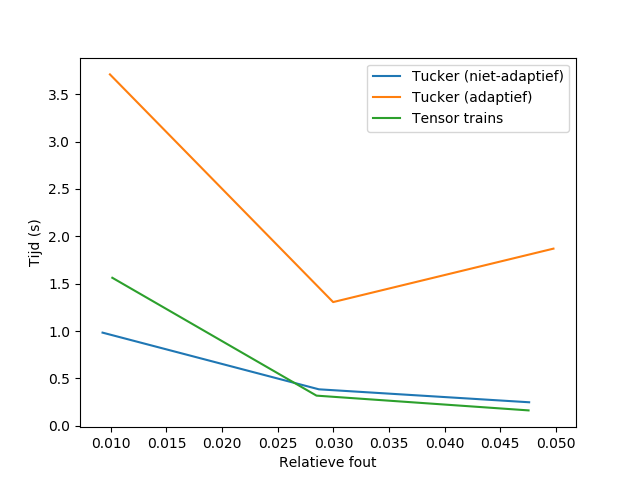
\includegraphics[width=\linewidth]{images/tucker_vs_tensor_trains_times_Indian_Pines.png}
  \caption{Indian Pines}
\end{subfigure}
\begin{subfigure}{0.48\textwidth}
  \centering
  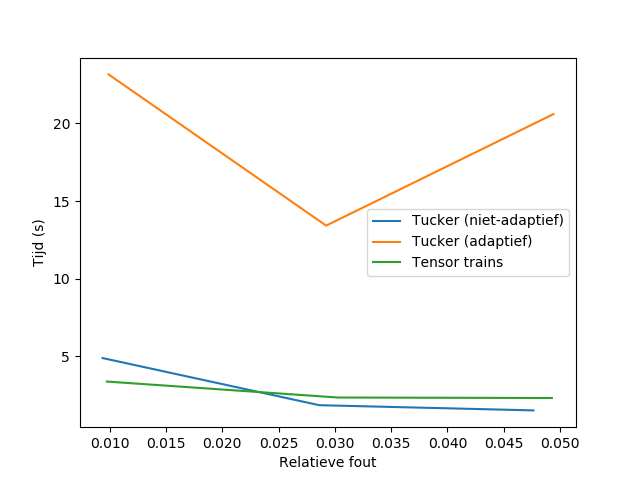
\includegraphics[width=\linewidth]{images/tucker_vs_tensor_trains_times_Cuprite.png}
  \caption{Cuprite}
\end{subfigure}
\\
\begin{subfigure}{0.48\textwidth}
  \centering
  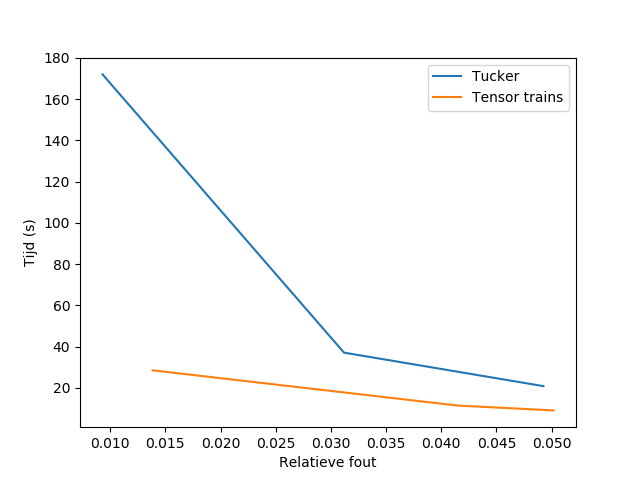
\includegraphics[width=\linewidth]{images/tucker_vs_tensor_trains_times_Pavia_Centre.png}
  \caption{Pavia Centre}
\end{subfigure}
\begin{subfigure}{0.48\textwidth}
  \centering
  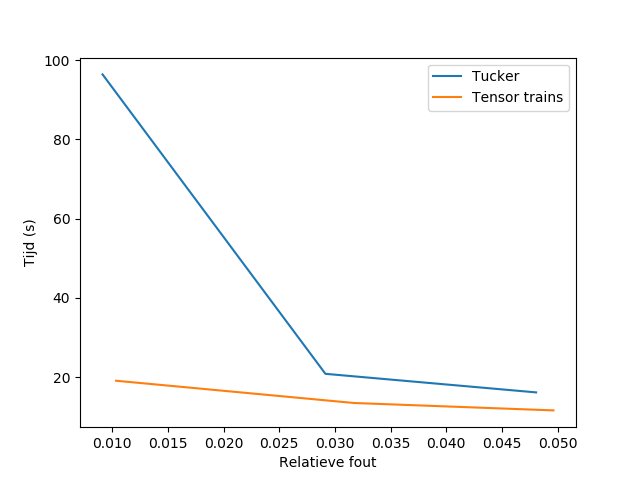
\includegraphics[width=\linewidth]{images/tucker_vs_tensor_trains_times_Mauna_Kea.png}
  \caption{Mauna Kea}
\end{subfigure}
\caption{Compressietijd in functie van relatieve fout voor Tucker-compressie en tensor trains (uitgemiddeld over 3 experimenten).}
\label{fig:tucker-vs-tensor-trains-times}
\end{figure}

\section{Vergelijking met algemene lossy compressie}

In deze sectie zullen we kort enkele algemene lossy-compressie-methoden bespreken, gevolgd door een vergelijking met onze tensor-train-gebaseerde compressie.

\newpage
\subsection{JPEG}

We hebben JPEG \cite{ref:jpeg} al aangehaald in hoofdstuk \ref{hoofdstuk:achtergrond}, maar nu leggen we uit hoe men hiermee een simpel algoritme kan maken voor het comprimeren van hyperspectrale afbeeldingen. Eerst verschuiven en schalen we de originele data, gevolgd door afronding, zodat elke waarde zich bevindt in het domein $\{0, 1, \dots, 255\}$. Deze quantisatie cre\"eert een fout die verwaarloosbaar is voor onze toepassingen. Daarna splitsen we de spectrale banden op in groepen van drie, comprimeren elke groep als \'e\'en RGB-afbeelding met JPEG en slaan de reeks gecomprimeerde afbeeldingen op. Bij de compressie wordt een kwaliteitsparameter opgegeven tussen 1 (slechtste kwaliteit) en 95 (beste kwaliteit). Deze methode houdt alleen rekening met de correlatie tussen de spectrale banden binnen elke groep, waardoor erg veel redundantie niet benut wordt en men geen goede compressie moet verwachten.

\newpage
\subsection{Videocompressie met x264}

Een betere manier om met algemene compressie de correlatie tussen de spectrale banden te gebruiken, is aan de hand van videocompressie. Een typische video bestaat namelijk uit een reeks \textit{frames} waarbij opeenvolgende frames erg op elkaar lijken, terwijl hyperspectrale afbeeldingen bestaan uit een reeks spectrale banden die allemaal qua structuur op elkaar lijken. Bovendien heeft videocompressie erg belangrijke toepassingen en wordt er al decennia met veel aandacht onderzoek gedaan in dit domein, dus men kan zich voorstellen dat moderne \textit{video codecs} erg effici\"ent zijn.\\

Concreet zullen we (zoals bij de JPEG-methode) eerst de volledige tensor quantiseren naar 8 bits, waarna we elke spectrale band doorgeven als een frame aan ffmpeg \cite{ref:ffmpeg}, een uitgebreid en veel-gebruikt programma voor het verwerken van audio en video. Voor de compressie gebruiken we de video codec x264 \cite{ref:x264}. Deze compressie gebeurt op basis van de CRF-parameter (\textit{constant rate factor}), die de afweging tussen de compressiefout en de grootte van de uitvoer bepaalt. Een CRF-waarde van 0 komt neer op lossless compressie, een waarde van 51 (het maximum) geeft de slechtste kwaliteit. Daarnaast heeft ffmpeg ook een preset-parameter, die bepaalt hoe belangrijk de compressietijd is ten opzichte van de compressiefactor en -fout. We zullen hiervoor zowel de standaardoptie \textit{medium} als de snelste optie \textit{ultrafast} proberen.

\subsection{Vergelijking}

In figuren \ref{fig:general-comparison-indian-pines}, \ref{fig:general-comparison-cuprite}, \ref{fig:general-comparison-pavia-centre} en \ref{fig:general-comparison-mauna-kea} zien we de algemene vergelijkingen op vlak van compressiefout en -factor. Zoals verwacht doet de JPEG-methode het erg slecht, dus hier zullen we verder geen rekening mee houden. Videocompressie aan de hand van x264 met preset medium scoort echter wel hoog en geeft ongeveer even goede compressie als tensor trains. Aan de andere kant zien we dat de preset ultrafast veel slechtere resultaten geeft. De resultaten van Tucker-gebaseerde compressie zijn weer even goed tot slechter dan bij tensor trains, zoals besproken in de vorige sectie, waar we ook al leerden dat deze methode trager was. Het is dus de vraag wat de verschillen in compressietijd tussen tensor trains en videocompressie dan zijn.\\

Het antwoord hierop vindt men in figuur \ref{fig:general-comparison-times}. Als het gaat om videocompressie zijn de resultaten consistent: de preset ultrafast is elke keer significant sneller dan medium. Daarnaast heeft de CRF-parameter ook slechts een beperkte invloed op de compressietijd. Dit ligt anders bij tensor trains: we merken dat de compressietijd hierbij sterker daalt in functie van de relatieve fout. Daarnaast zijn tensor trains sneller dan videocompressie voor goed comprimeerbare datasets (zie Cuprite en Mauna Kea) maar trager voor slecht comprimeerbare (zie Pavia Centre). Als men deze twee zaken combineert, kan men concluderen dat de compressietijd van onze methode met tensor trains sterk afhankelijk is van de grootte van de uitvoer van de ST-HOSVD en dat een significante hoeveelheid tijd besteed wordt aan het quantiseren en encoderen van deze uitvoer.

\newpage
\begin{figure}[H]
  \centering
  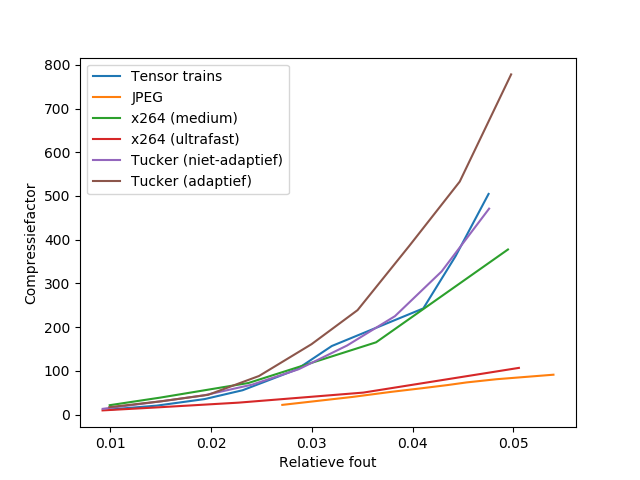
\includegraphics[scale=0.7]{images/general_comparison_new_Indian_Pines.png}
  \caption{Vergelijking tussen tensor trains en algemene compressiemethoden voor Indian Pines.}
\label{fig:general-comparison-indian-pines}
\end{figure}

\begin{figure}[H]
  \centering
  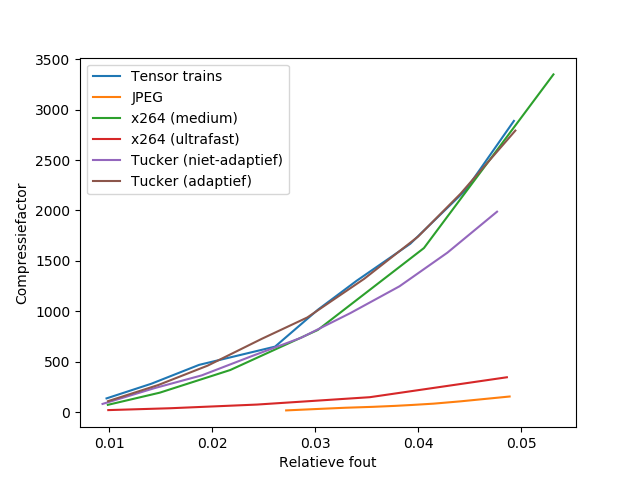
\includegraphics[scale=0.7]{images/general_comparison_new_Cuprite.png}
  \caption{Vergelijking tussen tensor trains en algemene compressiemethoden voor Cuprite.}
\label{fig:general-comparison-cuprite}
\end{figure}

\begin{figure}[H]
  \centering
  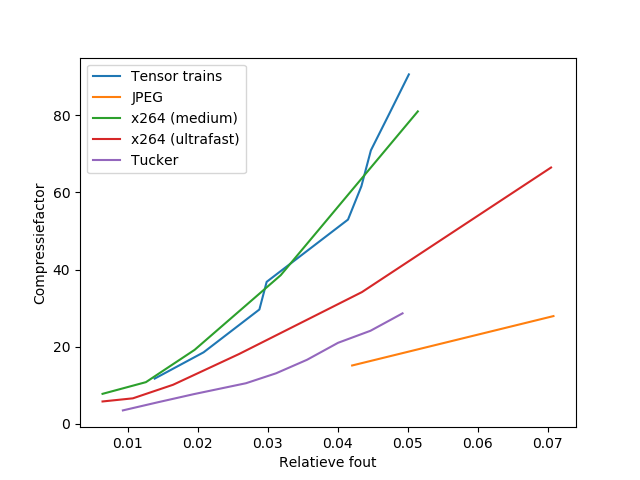
\includegraphics[scale=0.7]{images/general_comparison_new_Pavia_Centre.png}
  \caption{Vergelijking tussen tensor trains en algemene compressiemethoden voor Pavia Centre.}
\label{fig:general-comparison-pavia-centre}
\end{figure}

\begin{figure}[H]
  \centering
  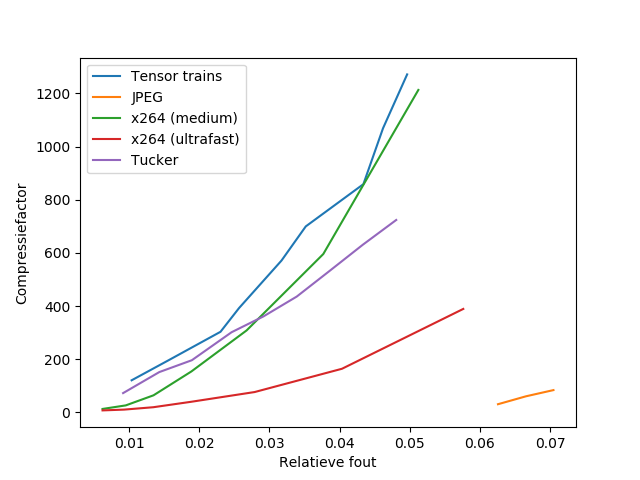
\includegraphics[scale=0.7]{images/general_comparison_new_Mauna_Kea.png}
  \caption{Vergelijking tussen tensor trains en algemene compressiemethoden voor Mauna Kea.}
\label{fig:general-comparison-mauna-kea}
\end{figure}

\begin{figure}[H]
\centering
\begin{subfigure}{0.48\textwidth}
  \centering
  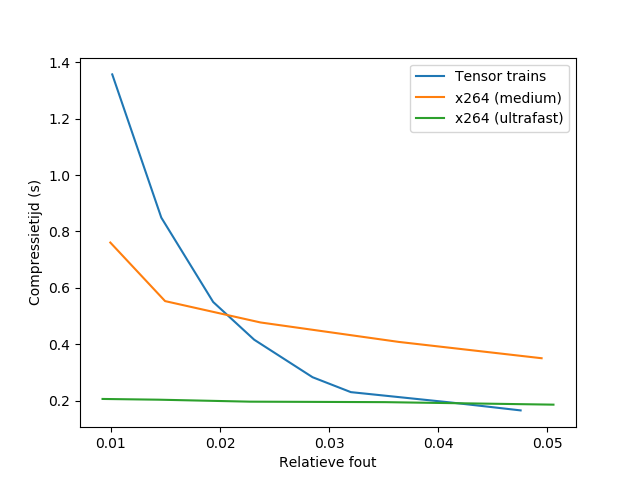
\includegraphics[width=\linewidth]{images/general_comparison_times_Indian_Pines.png}
  \caption{Indian Pines}
\end{subfigure}
\begin{subfigure}{0.48\textwidth}
  \centering
  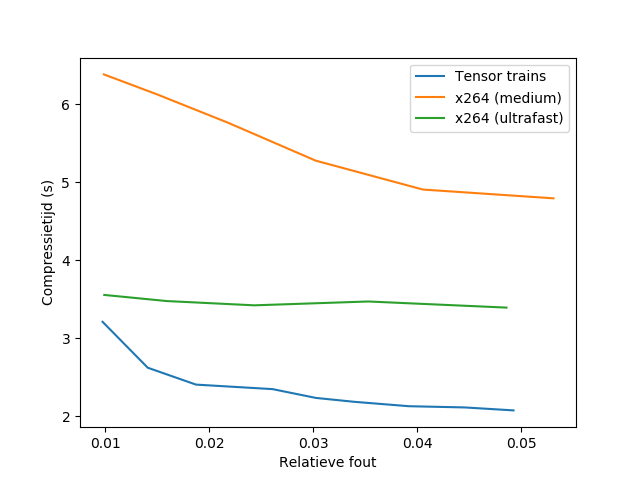
\includegraphics[width=\linewidth]{images/general_comparison_times_Cuprite.png}
  \caption{Cuprite}
\end{subfigure}
\\
\begin{subfigure}{0.48\textwidth}
  \centering
  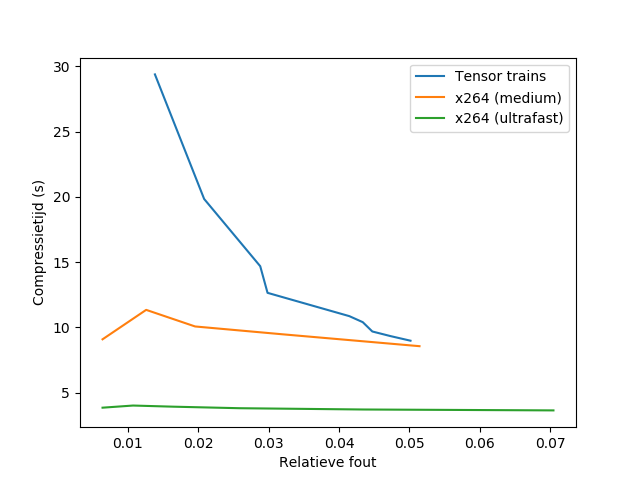
\includegraphics[width=\linewidth]{images/general_comparison_times_Pavia_Centre.png}
  \caption{Pavia Centre}
\end{subfigure}
\begin{subfigure}{0.48\textwidth}
  \centering
  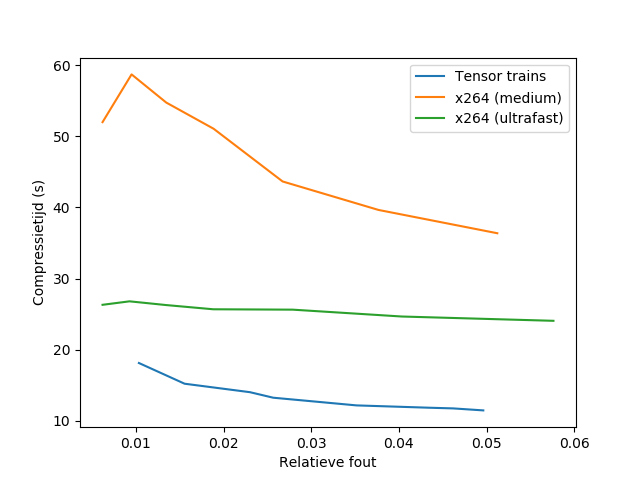
\includegraphics[width=\linewidth]{images/general_comparison_times_Mauna_Kea.png}
  \caption{Mauna Kea}
\end{subfigure}
\caption{Compressietijd in functie van relatieve fout voor tensor trains en videocompressie (uitgemiddeld over 10 experimenten).}
\label{fig:general-comparison-times}
\end{figure}

Onthoud wel dat deze vergelijking op \'e\'en core gebeurde. Als men gaat paralleliseren (wat men normaal gezien doet bij videocompressie), zullen tensor trains waarschijnlijk relatief slechter scoren omdat ons algoritme eerder sequentieel ontworpen is.\\

Ten slotte besloten we om ook eens te kijken naar de decompressietijd in figuur \ref{fig:general-comparison-decompression-times}. Opnieuw is de uitvoeringstijd van tensor trains erg afhankelijk van de relatieve fout, terwijl dit bij videocompressie minder invloed heeft. Verder heeft, zoals verwacht, de preset van ffmpeg erg weinig effect op de decompressietijd; deze parameter is namelijk alleen bedoeld om de compressietijd te controleren. We concluderen dat videocompressie over het algemeen veel sneller kan decomprimeren, maar dit verschil wordt kleiner bij grote datasets (zie Mauna Kea).

\newpage
\begin{figure}[H]
\centering
\begin{subfigure}{0.48\textwidth}
  \centering
  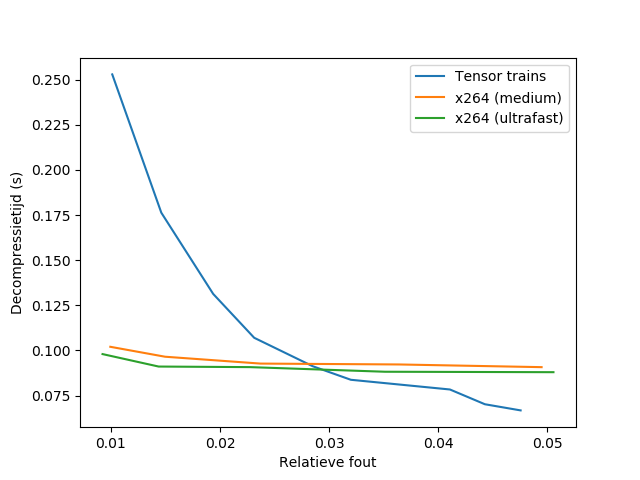
\includegraphics[width=\linewidth]{images/general_comparison_decompression_times_Indian_Pines.png}
  \caption{Indian Pines}
\end{subfigure}
\begin{subfigure}{0.48\textwidth}
  \centering
  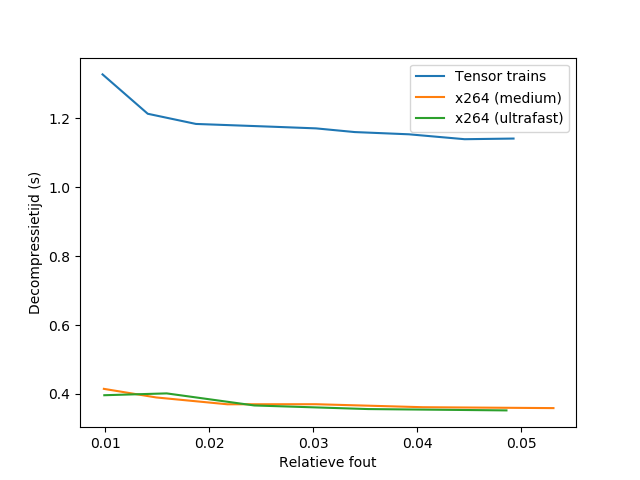
\includegraphics[width=\linewidth]{images/general_comparison_decompression_times_Cuprite.png}
  \caption{Cuprite}
\end{subfigure}
\\
\begin{subfigure}{0.48\textwidth}
  \centering
  \includegraphics[width=\linewidth]{images/general_comparison_decompression_times_Pavia_Centre.png}
  \caption{Pavia Centre}
\end{subfigure}
\begin{subfigure}{0.48\textwidth}
  \centering
  \includegraphics[width=\linewidth]{images/general_comparison_decompression_times_Mauna_Kea.png}
  \caption{Mauna Kea}
\end{subfigure}
\caption{Decompressietijd in functie van relatieve fout voor tensor trains en videocompressie (uitgemiddeld over 10 experimenten).}
\label{fig:general-comparison-decompression-times}
\end{figure}

\section{Vergelijking met de literatuur}

Aangezien hyperspectrale afbeeldingscompressie een klein onderzoeksdomein is en de gebruikte datasets meestal erg beknopt beschreven worden, is het moeilijk om veel concrete vergelijkingspunten te vinden in de literatuur. Om deze redenen zullen we ons beperken tot slechts \'e\'en ander resultaat: de paper van Karami et al. \cite{ref:karami}, die we al eerder aanhaalden bij de literatuurstudie in hoofdstuk \ref{hoofdstuk:achtergrond}. Zelfs hierbij wordt de voorverwerking van de data ook te kort besproken om de volgende vergelijking volledig te kunnen vertrouwen, maar we hebben alles geprobeerd om deze zo waarheidsgetrouw mogelijk voor te stellen.

\newpage
Karami et al. drukken de compressiefout uit als \textit{signal-to-noise ratio} (SNR) en de compressiegrootte uit als de \textit{rate} in bits per pixel per band. We zullen onze eigen resultaten omzetten met de volgende formules:
\[
SNR \text{ (in dB)} = -20 \log_{10}(\text{relatieve fout})
\]
\[
rate = \frac{\text{aantal bits per pixel per band in origineel}}{\text{compressiefactor}}
\]

\begin{figure}[H]
\begin{subfigure}{\textwidth}
  \centering
  \includegraphics[width=0.9\linewidth]{images/karami_edited_cuprite.png}
  \caption{De Cuprite-radiantie-dataset van Karami et al. \cite{ref:aviris_standard}.}
\end{subfigure}
\\
\begin{subfigure}{\textwidth}
  \centering
  \includegraphics[width=0.9\linewidth]{images/karami_edited_moffet_field.png}
  \caption{De Moffett-Field-radiantie-dataset van Karami et al. \cite{ref:aviris_standard}.}
\end{subfigure}
\caption{Vergelijking tussen tensor trains, videocompressie met x264 (preset medium) en de compressiemethoden van Karami et al. Deze grafieken zijn een aangepaste versies van de originelen uit hun paper \cite{ref:karami}.}
\label{fig:literature-comparison}
\end{figure}

\newpage
In figuur \ref{fig:literature-comparison} vindt men een vergelijking van de beste eerder besproken technieken (tensor trains en x264 met preset medium) en de technieken van Karami et al. Merk op dat hun domein anders ligt dan hetgene waarvoor wij onze algoritmen afgesteld hebben (de relatieve fouten van de tensor-train-metingen gaan hier van ongeveer 0.003 tot 0.03 in plaats van 0.01 tot 0.05). We zien dat hun methode het erg goed doet op de Cuprite-radiantie-dataset, maar bij de Moffett-Field-radiantie-dataset doet videocompressie het voor een groot deel van het domein beter. Ook tensor-train compressie scoort hier even goed tot significant beter voor bepaalde fouten.

\section{Voorbeeldcompressies}

Om dit hoofdstuk af te sluiten zullen we nog een aantal hyperspectrale afbeeldingen tonen voor en na compressie met tensor trains. Zoals in hoofdstuk \ref{hoofdstuk:methodologie} zullen we deze voorstellen door de spectrale banden op te tellen en deze sommen te verschuiven en schalen naar het domein $\{0, \dots, 255\}$. In deze sectie zullen relatieve fout en compressiefactor afgekort worden tot RF en CF respectievelijk.

\begin{figure}[H]
\centering
\begin{subfigure}{0.48\textwidth}
  \centering
  \includegraphics[scale=1]{images/indian_pines_cropped_sum.png}
  \caption{Origineel, 8910KB}
\end{subfigure}
\begin{subfigure}{0.48\textwidth}
  \centering
  \includegraphics[scale=1]{images/example_compression_Indian_Pines_0_01.png}
  \caption{RF: 0.0101, CF: 12.15, 733.3KB}
\end{subfigure}
\\
\begin{subfigure}{0.48\textwidth}
  \centering
  \includegraphics[scale=1]{images/example_compression_Indian_Pines_0_025.png}
  \caption{RF: 0.0231, CF: 55.89, 159.4KB}
\end{subfigure}
\begin{subfigure}{0.48\textwidth}
  \centering
  \includegraphics[scale=1]{images/example_compression_Indian_Pines_0_05.png}
  \caption{RF: 0.0475, CF: 504.75, 17.7KB}
\end{subfigure}
\caption{Voorbeeldcompressies van Indian Pines \cite{ref:ehu_aviris_indian_pines}.}
\end{figure}

\begin{figure}[]
\centering
\begin{subfigure}{\textwidth}
  \centering
  \includegraphics[scale=0.55]{images/cuprite_cropped_sum.png}
  \caption{Origineel, 103455KB}
\end{subfigure}
\\
\begin{subfigure}{\textwidth}
  \centering
  \includegraphics[scale=0.55]{images/example_compression_Cuprite_0_01.png}
  \caption{RF: 0.0098, CF: 136.2, 759.3KB}
\end{subfigure}
\end{figure}
\begin{figure}[]
\centering
\ContinuedFloat
\begin{subfigure}{\textwidth}
  \centering
  \includegraphics[scale=0.55]{images/example_compression_Cuprite_0_025.png}
  \caption{RF: 0.0261, CF: 649.6, 159.3KB}
\end{subfigure}
\begin{subfigure}{\textwidth}
  \centering
  \includegraphics[scale=0.55]{images/example_compression_Cuprite_0_05.png}
  \caption{RF: 0.0493, CF: 2888.5, 35.8KB}
\end{subfigure}
\caption{Voorbeeldcompressies van Cuprite \cite{ref:ehu_aviris_cuprite}.}
\end{figure}

\begin{figure}[]
\centering
\begin{subfigure}{\textwidth}
  \centering
  \includegraphics[width=0.85\linewidth]{images/pavia_sum.png}
  \caption{Origineel, 146657.7KB}
\end{subfigure}
\end{figure}
\begin{figure}[]
\centering
\ContinuedFloat
\begin{subfigure}{\textwidth}
  \centering
  \includegraphics[width=0.85\linewidth]{images/example_compression_Pavia_Centre_0_01.png}
  \caption{RF: 0.0138, CF: 11.67, 12569.8KB}
\end{subfigure}
\end{figure}
\begin{figure}[]
\centering
\ContinuedFloat
\begin{subfigure}{\textwidth}
  \centering
  \includegraphics[width=0.85\linewidth]{images/example_compression_Pavia_Centre_0_025.png}
  \caption{RF: 0.0298, CF: 36.8, 3985.7KB}
\end{subfigure}
\end{figure}
\begin{figure}[]
\centering
\ContinuedFloat
\begin{subfigure}{\textwidth}
  \centering
  \includegraphics[width=0.85\linewidth]{images/example_compression_Pavia_Centre_0_05.png}
  \caption{RF: 0.0502, CF: 90.7, 1617.6KB}
\end{subfigure}
\caption{Voorbeeldcompressies van Pavia Centre \cite{ref:ehu_rosis}.}
\end{figure}

\begin{figure}[]
\centering
\begin{subfigure}{0.48\textwidth}
  \centering
  \includegraphics[width=0.8\linewidth]{images/mauna_kea_sum.png}
  \caption{Origineel, 766156.2KB}
\end{subfigure}
\begin{subfigure}{0.48\textwidth}
  \centering
  \includegraphics[width=0.8\linewidth]{images/example_compression_Mauna_Kea_0_01.png}
  \caption{RF: 0.0104, CF: 121, 6332.1KB}
\end{subfigure}
\end{figure}
\begin{figure}[]
\centering
\ContinuedFloat
\begin{subfigure}{0.48\textwidth}
  \centering
  \includegraphics[width=0.8\linewidth]{images/example_compression_Mauna_Kea_0_025.png}
  \caption{RF: 0.0257, CF: 392.67, 1951.2KB}
\end{subfigure}
\begin{subfigure}{0.48\textwidth}
  \centering
  \includegraphics[width=0.8\linewidth]{images/example_compression_Mauna_Kea_0_05.png}
  \caption{RF: 0.0496, CF: 1271.31, 602.7KB}
\end{subfigure}
\caption{Voorbeeldcompressies van Mauna Kea \cite{ref:aviris}.}
\end{figure}

\chapter{Besluit}
\label{hoofdstuk:besluit}

De masterproeftekst wordt afgesloten met een hoofdstuk waarin alle
besluiten nog eens samengevat worden. Dit is ook de plaats voor suggesties
naar het verder gebruik van de resultaten, zowel industri"ele toepassingen
als verder onderzoek.




% Indien er bijlagen zijn:
\appendixpage*          % indien gewenst
\appendix
\chapter{Code algoritmen}
\label{app:algoritmen}

\section{\texttt{st\_hosvd.py}}

Ondanks de naam, bevat dit bestand code omtrent alle algoritmen besproken in hoofdstuk \ref{hoofdstuk:tucker}, niet alleen de ST-HOSVD.\\

\lstinputlisting[style=Python]{../code/st_hosvd.py}
\chapter{Code voorverwerker}
\label{app:voorverwerker}

Zet hier script om data te pre-processen. TODO
\chapter{Code \texttt{bitarray}}
\label{app:bitarray}

Deze bijlage beperkt zich tot slechts tot de toegevoegde stukken code uit \texttt{\_bitarray.c}.\\

\lstinputlisting[style=C,linerange={2318-2382},firstnumber=2318]{../code/bitarray/bitarray/_bitarray.c}
\lstinputlisting[style=C,linerange={2489-2531},firstnumber=2489]{../code/bitarray/bitarray/_bitarray.c}
\lstinputlisting[style=C,linerange={2599-2726},firstnumber=2599]{../code/bitarray/bitarray/_bitarray.c}
\lstinputlisting[style=C,linerange={2845-2950},firstnumber=2845]{../code/bitarray/bitarray/_bitarray.c}

\backmatter
% Na de bijlagen plaatst men nog de bibliografie.
% Je kan de  standaard "abbrv" bibliografiestijl vervangen door een andere.
\bibliographystyle{abbrv}
\bibliography{referenties}

\end{document}

%%% Local Variables: 
%%% mode: latex
%%% TeX-master: t
%%% End: 
